%&<tex>
\documentclass[notheorems,xcolor=dvipsnames]{beamer}
\usetheme{Rochester}
%\usefonttheme{serif}

%\usepackage[hmargin=2.5cm, vmargin=2cm]{geometry}
\usepackage{amssymb, mathtools, yhmath, graphicx}
\usepackage{standalone}
\usepackage[most]{tcolorbox}
%\usepackage{fontspec, type1cm, titlesec, titling, fancyhdr, tabularx}
%\usepackage{unicode-math}
\usepackage{float}
\usepackage{transparent}
\usepackage[normalem]{ulem}
\usepackage{bm}
\usepackage{array}
\usepackage{csquotes}
\usetikzlibrary{arrows}
\usepackage{soul}
\usepackage[normalem]{ulem}

%\usepackage{eulervm}

\usepackage{xpatch}
\usepackage{relsize}
\usepackage{scalerel}
\usepackage{stackengine}
\usepackage{gauss}
%\usepackage[abbreviations, per-mode=symbol]{siunitx}
\usepackage[CheckSingle, CJKmath]{xeCJK}
\usepackage{fontspec}
\defaultfontfeatures{Mapping=tex-text}
\usefonttheme{professionalfonts}
\usepackage{concmath}
%\usepackage{CJKulem}
%\usepackage{enumitem}
\usepackage{tikz}
\usetikzlibrary{calc, fit, backgrounds}
\usetikzlibrary{tikzmark}
\tikzset {
  overlay node/.style={
    anchor=base, outer sep=0mm, inner sep=0mm,
  }
}
\usepackage{minted}
% \usepackage{python}
% \usepackage{algorithm2e}
\definecolor{mgray}{rgb}{0.85, 0.85, 0.85}
\colorlet{mgreen}{green!70!black}
\newmintinline{cpp}{bgcolor=mgray}
\def\codesize{\fontsize{9}{12}\selectfont}
\setmonofont[Mapping=]{Source Code Pro}
%\setmonofont[Contextuals={Alternate}]{Fira Code}
\setminted{fontsize=\codesize, linenos, frame=lines, mathescape, autogobble}
%\usemintedstyle{monokai}
%\usepackage{circuitikz}
%\setCJKmainfont[BoldFont=cwTex Q Hei]{cwTex Q Ming}
%\setCJKsansfont[BoldFont=cwTex Q Hei]{cwTex Q Ming}
%\setCJKmonofont[BoldFont=cwTex Q Hei]{cwTex Q Ming}
\setCJKmainfont[AutoFakeSlant,BoldFont=Source Han Sans TW Bold]{Noto Sans CJK TC}
\newfontfamily\SHSTW{Source Han Sans TW}

\def\ofootnotesize{\fontsize{8}{12}}
\def\footnotesize{\fontsize{6}{8}\selectfont}
%\def\normalsize{\fontsize{12}{18}\selectfont}
%\def\large{\fontsize{14}{21}\selectfont}
%\def\Large{\fontsize{16}{24}\selectfont}
%\def\LARGE{\fontsize{18}{27}\selectfont}
%\def\huge{\fontsize{20}{30}\selectfont}

%\titleformat{\section}{\bf\Large}{\arabic{section}}{24pt}{}
%\titleformat{\subsection}{\large}{\arabic{subsection}.}{12pt}{}
%\titlespacing*{\subsection}{0pt}{0pt}{1.5ex}

%\usepackage{parskip}
%\parindent=24pt
%\parskip=1em

\setlength{\parskip}{\baselineskip} 
\usepackage{trimclip}
\DeclareRobustCommand\Longrightarrow{\NewRelbar\joinrel\Rightarrow}
\DeclareRobustCommand\Longleftarrow{\Leftarrow\joinrel\NewRelbar}

\makeatletter
\DeclareRobustCommand\NewRelbar{%
  \mathrel{%
    \mathpalette\@NewRelbar{}%
  }%
}
\newcommand*\@NewRelbar[2]{%
  % #1: math style
  % #2: unused
  \sbox0{$#1=$}%
  \sbox2{$#1\Rightarrow\m@th$}%
  \sbox4{$#1\Leftarrow\m@th$}%
  \clipbox{0pt 0pt \dimexpr(\wd2-.6\wd0) 0pt}{\copy2}%
  \kern-.2\wd0 %
  \clipbox{\dimexpr(\wd4-.6\wd0) 0pt 0pt 0pt}{\copy4}%
}
\makeatother



\newcommand{\img}{\mathsf{i}}
\newcommand{\ex}{\mathsf{e}}
\newcommand{\dD}{\mathrm{d}}
\newcommand{\dI}{\,\mathrm{d}}
\newcommand{\linearprog}[3][maximize]{%
\begin{array}{rl}
  \text{#1} & \kern 1em {#2} \\[8pt]
  \text{subject to} & {\renewcommand\arraystretch{1.1} #3}
\end{array}%
}

\newcommand\abs[1]{\left\lvert #1 \right\rvert}
\newcommand{\ord}{\mathcal{O}}
\newcommand{\fourier}{\mathcal{F}}
\newcommand*{\defeq}{\triangleq}
\renewcommand*{\sharp}{\mathlarger{\#}}
\newcommand*{\bZ}{\mathbb{Z}}
\newcommand*{\bF}{\mathbb{F}}
\newcommand*{\correspond}{\mathrel{\stackon[1.5pt]{=}{\stretchto{%
    \scalerel*[\widthof{=}]{\wedge}{\rule{1ex}{3ex}}}{0.5ex}}}}
\newcommand*{\Expect}{{\rm I\kern-.3em E}}
\newcommand{\btitle}[1]{{\secname} -- #1}
\newcommand{\disskip}[1][1]{\vspace*{-#1\parskip}}%
\renewcommand*{\sharp}{\mathlarger{\#}}
\newcommand{\tikzoverlay}[2]{\tikz[baseline, remember picture]{ \node[overlay node] (#1) {#2}}}%

\theoremstyle{definition}
\newtheorem{theorem}{定理}
\newtheorem{lemma}{引理}
\newtheorem{property}{性質}
\newtheorem{corollary}{推論}
\newtheorem{conjecture}{猜想}
\newtheorem{problem}{題目}

%\colorlet{origintitlefg}{block title.fg}
%\setbeamercolor{origintitle}{use=block,fg=block title.fg,bg=block title.bg}
%\setbeamercolor{originbody}{use=block body,fg=block body.fg,bg=block body.bg}

\newtheorem{definition}{定義}
\BeforeBeginEnvironment{definition}{%
  \setbeamercolor{block title}{fg=white,bg=red!70!black}
  \setbeamercolor{block body}{fg=black, bg=block title.bg!10!bg}
}
\AfterEndEnvironment{definition}{
    \setbeamercolor{block title}{use=structure,fg=white,bg=structure.fg!75!black}
    \setbeamercolor{block body}{parent=normal text,use=block title,bg=block title.bg!10!bg}
}

\newenvironment{missue}{%
\setbeamercolor{block title}{bg=ForestGreen,fg=white}
\setbeamercolor{block body}{bg=blue!20!green!20,fg=black}
\begin{block}{\centering 問題}}{\end{block}}

\newenvironment{exercise}{%
\setbeamercolor{block title}{bg=ForestGreen,fg=white}
\setbeamercolor{block body}{bg=blue!20!green!20,fg=black}
\begin{block}{習題}}{\end{block}}

\renewenvironment{proof}{%
\begin{tcolorbox}[frame empty] {\bf 證明:}\ }{\end{tcolorbox}}

%\setbeamercovered{transparent}
%\usefonttheme[onlymath]{serif}
%\settowidth{\leftmargini}{\usebeamertemplate{itemize item}}

%\makeatletter
%\patchcmd\beamer@@tmpl@frametitle{\insertframetitle}{\insertsection-\insertframetitle}{}{}
%\makeatother

\setbeamertemplate{enumerate item}{%
  \usebeamercolor[bg]{item projected}%
  \raisebox{0.28ex}{\colorbox{bg}{\color{fg}\scriptsize\insertenumlabel}}%
}

\setbeamertemplate{itemize item}{%
  \usebeamercolor[bg]{item projected}%
  \raisebox{0.25ex}{\scriptsize$\blacksquare$}%
}

\AtBeginSection[]{
  \begin{frame}
    \tableofcontents[currentsection]
  \end{frame}
  \begin{frame}
  \vfill
  \centering
  \begin{beamercolorbox}[sep=6pt,center,shadow=true,rounded=true]{title}
    \usebeamerfont{title}\LARGE\insertsectionhead\par%
  \end{beamercolorbox}
  \vfill
  \end{frame}

}

\makeatletter
\let\save@measuring@true\measuring@true
\def\measuring@true{%
  \save@measuring@true
  \def\beamer@sortzero##1{\beamer@ifnextcharospec{\beamer@sortzeroread{##1}}{}}%
  \def\beamer@sortzeroread##1<##2>{}%
  \def\beamer@finalnospec{}%
}
\makeatother

\title{基礎動態規劃}
\author{yp155136}

\renewcommand*{\emph}[1]{{\bfseries #1}}

\begin{document}

\begin{frame}
  \titlepage
\end{frame}

\begin{frame}{講師簡介}
  \begin{itemize}
    \item yp155136
    \item LYB / BBCube
    \begin{itemize}
      \item ICPC 2021 台北站第二名
      \item ICPC 2019 雅加達站第四名
    \end{itemize}
    \item IOI 2018 國際資訊奧林匹亞銀牌
    \item APIO 2018 亞太資訊奧林匹亞金牌
    \only<2> {
    \item 因為想學習基礎 DP 所以當基礎 DP 講師
    }
  \end{itemize}
\end{frame}

% \begin{frame}{大綱}
%   \tableofcontents
% \end{frame}
\begin{frame}{大綱}
  \begin{itemize}
    \item 單調隊列優化
    \item 斜率優化
    \item 凹凸單調優化
    \item Knuth Optimization
    \item 轉移點單調優化
    \item SMAWK 演算法
    \item Aliens 優化
  \end{itemize}
\end{frame}

\begin{frame}{前言}
  \begin{itemize}
    \item 相信大家已經具備基本的 DP 能力了
    \item 基礎 DP 這節課,是要教大家許多 DP 優化的技巧
    \item 大家可以想像 DP 優化是一個工具,用來幫助你更快的計算 DP 式子
  \end{itemize}
\end{frame}

\documentclass[standalone]{beamer}

\begin{document}
\section{單調隊列優化}

\begin{frame}{\btitle{例題}}
  \begin{problem}[ZJ a146 Sliding Window]
    給定一個長度為 $N$ 的序列 $A$ 以及一個整數 $K$,請找出所有長度為 $K$ 的窗口極值。也就是說,對於所有的 $K \leq i \leq N$,求出 $\min_{i - K + 1 \leq j \leq i}A_j$ 以及 $\max_{i - K + 1 \leq j \leq i}A_j$。

    \begin{itemize}
      \item $N, K \leq 10^6$
    \end{itemize}

    比如說,如果 $A = (4, 3, 5, 1, 6), K = 3$,那你要分別輸出 $(5, 5, 6)$ 跟 $(3, 1, 1)$
  \end{problem}
\end{frame}

\begin{frame}{單調隊列優化}
  \begin{itemize}
    \item naive 作法:$O(NK)$,太慢了
    \item 用線段樹等等資料結構硬砸,雖然是 $O(N \log N)$,但還是不夠快
    \item 因此,我們需要一些觀察
    \item 假設我們在做 $\min$ 的情況
  \end{itemize}
\end{frame}

\begin{frame}{單調隊列優化}
  \begin{itemize}
    \item 假設我們已經計算完尾端是 $i$ 的答案
    \item 那,對所有 $j < i$,如果 $A_j > A_i$,那 $A_j$ 就永遠不可能是答案了
    \item $A = [9, 6, 2]$,在看到 $2$ 之後,$6$ 就不可能成為答案了
    \item 因此,我們可以維護一個結構,來儲存\textbf{目前有可能是答案的元素}
    \item 想想看,這個結構裡面的元素,應該是遞增的,還是遞減的?
  \end{itemize}
\end{frame}

\begin{frame}{單調隊列優化}
  \begin{itemize}
    \item 結構裡面的元素是遞增的
    \item 後面的元素,雖然目前暫時不是最佳解,\textbf{但是等到前面的元素過期(window 大小超過 K)的時候},就有可能變成最佳解了
    \item 算法結構如下:
    \begin{itemize}
      \item 每次要將 $i$ 放入之前,可以先從後面將所有大於 $A_i$ 的元素全部 pop 掉(因為被 pop 掉的元素不可能成為最佳解了)
      \item 每次計算答案的時候還需檢查在資料結構最前面(基於單調性,一定是目前裡面最小的元素)的元素是否還合法,不合法的話要 pop 掉
      \item 我們便可以確定此時資料結構最前的元素就是位置 $i$ 的答案
    \end{itemize}
  \end{itemize}
\end{frame}

\begin{frame}{單調隊列優化}
  假設 $A = [4, 6, 8, 7, 9, 1], K = 3$

  \begin{center}
    \begin{tabular}{|p{0.1\textwidth}|p{0.1\textwidth}|p{0.1\textwidth}|p{0.1\textwidth}|p{0.1\textwidth}|p{0.1\textwidth}|}
      \hline
      4 & 6 & 8 & 7 & 9 & 1 \\ [5ex]
      \hline
    \end{tabular}
  \end{center}
\end{frame}

\begin{frame}{單調隊列優化}
  \begin{itemize}
    \item 那個資料結構需要支援從前面刪除元素,從後面加入及刪除元素,雙向佇列(double-ended queue, deque)是一個不錯的選擇,且 STL 也有提供 \texttt{std::deque} 容器,不需要自己手寫。
  \end{itemize}
\end{frame}

\begin{frame}[fragile]{\btitle{範例程式碼}}
  \begin{minted}[breaklines]{cpp}
    void find_min(int n, int k) {
      deque<int> dq;
      for (int i = 1; i <= n; ++i) {
        while (!dq.empty() && a[dq.back()] > a[i]) dq.pop_back(); // 把所有大於 a[i] 的元素通通刪掉
        dq.push_back(i);
        if (dq.front() == i - k) dq.pop_front(); // 如果最前面的元素已經不合法(過期),就 pop 掉
        ans_mn[i] = a[dq.front()];
      }
    }
  \end{minted}
\end{frame}

\begin{frame}{單調隊列優化}
  \begin{itemize}
    \item 時間複雜度?$O(N^2)$?
    \item 均攤分析:考慮\textbf{總共的操作數量}(在這題來說就是看 \texttt{pop} 跟 \texttt{push} 的數量)
    \item \texttt{push} 至多 $N$ 次,因此也至多 \texttt{pop} $N$ 次
    \item 因此總操作數量為 $O(N)$,每個操作是均攤 $O(1)$ 的
    \item 因此,總操作的複雜度為 $O(N)$
  \end{itemize}
\end{frame}

\begin{frame}{\btitle{應用}}
  \begin{problem}[CF 372C Watching Fireworks is Fun]
    有 $M$ 個煙火將在一維數線上綻放。第 $i$ 個煙火在時間 $t_i$ 、於位置 $a_i$ 綻放,其中 $1 \leq a_i \leq N$。如果你在位置 $1 \leq x \leq N$ 觀看煙火 $i$ 的話,你會獲得 $b_i - |a_i - x|$ 的開心度。此外,你每秒可以移動 $d$ 單位的距離,且不能離開 $1$ 到 $N$ 的位置範圍。你可以任選初始位置,請問看完 $M$ 的煙火所獲得的總開心度最大能多少。

    \begin{itemize}
      \item $1 \leq M \leq 300$
      \item $1 \leq N \leq 1.5 \times 10^5$
    \end{itemize}
  \end{problem}
  先想想看 DP 式子要怎麼列,再看看能不能用單調隊列優化達到更好的複雜度
\end{frame}

\begin{frame}{\btitle{應用}}
  \begin{itemize}
    \item 首先將所有的煙火按照綻放的時間,由小到大排序好
    \item 令 $dp(i, j)$ 為看完第 $i$ 個煙火且位於位置 $j$ 的最大開心度
    \item $dp(0, i) = 0$ 對所有 $1 \leq i \leq N$
    \item $dp(i, j) = \max_{|k - j| \leq d \times (t_i - t_{i - 1})} dp(i - 1, k) + b_i - |a_i - j|$
    \item 注意到 $b_i - |a_i - j|$ 跟 $k$ 完全無關,所以重要的其實是求出所有在可到達範圍內的 $dp_{i - 1, k}$ 的最大值
    \item 由於 $|k - j| \leq d \times (t_i - t_{i - 1})$ 這個限制其實是 $\max(1, j - d \times (t_i - t_{i - 1}) \leq k \leq \min(N, j + d \times (t_i - t_{i - 1}))$,所以這個問題其實就是一個滑動窗口極值的計算
  \end{itemize}
\end{frame}

\begin{frame}{\btitle{應用}}
  \begin{problem}[有限個數的多重背包問題]
    有 $N$ 種物品,第 $i$ 種重量為 $w_i$,價值為 $v_i$,且總共有 $s_i$ 個。求選出若干個物品使得總重量不超過 $W$ 的情況下,最大總價值為何。
  \end{problem}

  最 Naive 的作法是 $O(NWK)$,如果用二進制拆解的話可以壓到 $O(NW \log K)$($K$ 是 $s_i$ 的最大值),有沒有辦法作到更好呢?
\end{frame}


\begin{frame}{\btitle{應用}}
  \begin{itemize}
    \item 令 $dp(i, j)$ 代表前 $i$ 種物品中,選出總重量為 $j$ 的最大價值和
    \item $dp(i, j) = \max_{0 \leq x \leq s_i}\left\{dp(i - 1, j - x \times w_i) + x \times v_i \right\}$
    \item $dp(i, j) = \max_{0 \leq \frac{j - k}{w_i} \leq s_i, j \equiv k \pmod w_i}\left\{dp(i - 1, k) + \frac{j - k}{w_i} \times v_i \right\}$
    \item $dp(i, j) = \lfloor\frac{j}{w_i}\rfloor \times v_i + \max_{0 \leq \frac{j - k}{w_i} \leq s_i, j \equiv k \pmod w_i}\left\{dp(i - 1, k) - \lfloor\frac{k}{w_i}\rfloor \times v_i \right\}$
    \item 如此一來,對於一個除以 $w_i$ 的餘數 $r$,上面的轉移式就是一個滑動窗口的極值問題,因此可以套用單調隊列的手法加速達到 $O(\text{除以 $w_i$ 餘 $r$ 的個數})$,對所有餘數取總和的話恰好就是 $O(W)$,於是有限背包問題便得到了 $O(NW)$ 的解法
  \end{itemize}
\end{frame}

\end{document}


\documentclass[standalone]{beamer}

\begin{document}
\section{斜率優化}

\begin{frame}{\btitle{形式}}
  \begin{itemize}
    \item 斜率優化又稱凸包優化(convex-hull optimization),幾乎是所有 DP 優化的技巧中,最常見也最容易套用的一種
    \item 常見的 DP 式子形式:$dp(i) = c_i + \max_{j \leq R_i} \{a_jx_i + b_j\}$
    \item 其中 $R_i$ 是一個遞增的序列,而 $c_i$ 是一個與取 max 沒有直接關係的項,可以視為不存在
    \item 通常來說 $a_j$ 或 $b_j$ 會包含 $dp(j)$ 的值,因此在這種情況下會額外的有 $R_i < i$ 的限制
  \end{itemize}
\end{frame}

\begin{frame}{斜率優化}
  \begin{itemize}
    \item 與剛才介紹的單調隊列優化很相似,對於兩個 $j, k$,如果有 $a_k > a_j$ 且 $a_kx + b_k > a_jx + b_j$
    \item 那麼對於所有的 $x^\prime > x$ 而言,$j$ 都不可能是最好的轉移來源
    \item 基於這個觀察,我們可以對已經算好的 $j \leq R_i$,都將 $a_jx + b_j$ 當成是二維平面上的一條直線畫出來
    \item 如此一來,我們的 DP 轉移就變成要查詢 $x_i$ 帶入這些線的最大值,以及要支援動態的將新的直線加入
    \item 先介紹斜率與查詢都是單調的版本,接下來才會進入斜率、查詢不單調的版本
  \end{itemize}
\end{frame}

\begin{frame}{\btitle{斜率、查詢單調}}
  \begin{problem}[ZJ a146 Sliding Window]
    現在你要過 $N$ 個關卡,關卡編號為 $1, 2, \dots, N$,每一個關卡都有一隻怪獸,第 $i$ 個關卡的怪獸的能力值為 $s_i$。在還沒進入任何關卡之前,你有一個初始的技能值 $x$。

    在第 $1, 2, \dots, N - 1$ 關卡中,你可以選擇打倒怪獸,或者是直接逃跑。如果你選擇打倒第 $i$ 隻怪獸,你要花 $f \times s_i$ 的時間打倒怪獸,其中 $f$ 是你當前的技能值。在打倒怪獸後,你的新的能力值會變成 $f_i$。

    你的最終目標是打倒第 $N$ 隻關卡的怪獸,請問在這個過程中,你最少需要花費多少時間。

    \begin{itemize}
      \item $N \leq 2 \times 10^5$
      \item $1 \leq s_1 \leq s_2 \leq \dots \leq s_N \leq 10^6$
      \item $x \geq f_1 \geq f_2 \dots \geq f_N \geq 1$
    \end{itemize}
  \end{problem}
\end{frame}

\begin{frame}{\btitle{斜率、查詢單調}}
  \begin{itemize}
    \item 假設 $f_0 = 0, dp(0) = 0$,應該不難列出以下的 DP 式子:
    \item $dp(i) = \min_{0 \leq j < i}(dp(j) + f_j \times s_i)$
    \item 為了之後講解方便,我們先把所有的 $f_i$ 設成 $-f_i$,我們就可以把 DP 式子轉換成取最大值的形式
    \item $dp(i) = \max_{0 \leq j < i}(dp(j) + f_j \times s_i)$
    \item 並且最後的答案為 $-dp(N)$
  \end{itemize}
\end{frame}

\begin{frame}{\btitle{斜率、查詢單調}}
  \begin{itemize}
    \item $dp(i) = \max_{0 \leq j < i}(dp(j) + f_j \times s_i)$
    \item 如果把上面那個 DP 式寫成斜率優化的形式
    \item 斜率 $a = f_j$,截距 $b = dp(j)$
    \item 轉移 $dp(i)$ 的時候,就是要查詢在 $x = s_i$ 的情況下,那些直線的最大值
    \item 特別的是,我們可以發現:查詢 $s_i$ 跟斜率 $f_j$ 都是\textbf{單調遞增}的
  \end{itemize}
\end{frame}

\begin{frame}{\btitle{斜率、查詢單調}}
  \begin{itemize}
    \item 因此,在這個條件下,這個轉移式會跟前面介紹的單調隊列優化有類似著性質
    \item 如果 $k < j$ 是 $i$ 的最佳轉移來源,那麼對於所有 $i < i^\prime$,從 $j$ 轉移一定會比從 $k$ 轉移來還的好
    \item $a_jx_i + b_j > a_kx_i + b_k \implies a_jx_{i^\prime} + b_j = a_jx_i + a_j(x_{i^\prime} - x_i) + b_j > a_kx_i + a_k(x_{i^\prime} - x_i) + b_k = a_kx_{i^\prime} + b_k$
    \item 有了這個性質以後,我們可以進一步的將時間複雜度壓低
  \end{itemize}
\end{frame}

\begin{frame}{\btitle{斜率、查詢單調}}
  \begin{itemize}
    \item 跟單調隊列一樣,我們維護一個直線的 deque,其中直線由頭至尾斜率遞增
    \item 每次轉移的時候我們可以考慮最前面兩個直線 $L_1, L_2$,比較是否有 $L_1(x_i) < L_2(x_i)$
    \item 根據上面的性質,如果成立的話則代表 $L_1$ 再也不可能成為之後的最佳轉移來源,所以可以將 $L_1$ 移除
    \item 重複這個動作直到現在 deque 最前面的元素 $L$ 還沒有被淘汰,則這時 $L$ 便會是 $i$ 最佳的轉移來源
  \end{itemize}
\end{frame}

\begin{frame}{\btitle{斜率、查詢單調}}
  \begin{itemize}
    \item 解決完查詢以後,接著必須也將加入直線的複雜度降低
    \item 由於斜率單調遞增,我們可以確定現在要加入的直線 $L^\prime$ 一定比現在 deque 中的直線斜率都還要大
    \item 而不難發現,$L^\prime$ 能淘汰的人會是 deque 尾端的一些\textbf{連續}的直線
    \item 假設現在 deque 中最後面的元素為 $L_{-1}$,倒數第二個為 $L_{-2}$
    \item 則可以發現,當 \textbf{$L^\prime$ 與 $L_{-1}$ 的交點比 $L_{-1}$ 以及 $L_{-2}$ 的交點還要左邊}時
    \item $L_{-1}$ 的有效區間會完全的被 $L^\prime$ 覆蓋,再也不可能成為轉移的候選人
  \end{itemize}
\end{frame}


\begin{frame}{\btitle{斜率、查詢單調}}
  \begin{figure}[H]
    \centering
    \begin{tikzpicture}[scale=0.3]
      \begin{scope}
      %\draw [domain=0:14,smooth,variable=\x,thick] plot ({\x}, {0.07142857142857142 * \x});
      \draw [domain=0:210/23,smooth,variable=\x,very thick] plot ({\x}, {0.07142857142857142 * \x});
      \draw [domain=210/23:14,smooth,variable=\x,gray] plot ({\x}, {0.07142857142857142 * \x});
      \draw [domain=0:210/23,smooth,variable=\x,gray] plot ({\x}, {0.4 * \x - 3});
      \draw [domain=210/23:14,smooth,variable=\x,very thick] plot ({\x}, {0.4 * \x - 3});
      \draw [domain=0:14,smooth,variable=\x,dashed] plot ({\x}, {0.9 * \x - 5.5});
      \node at (10, 6) (a1) {$L^\prime$};
      \node at (12, 3) (a2) {$L_{-1}$};
      \node at (2, 1) (a3) {$L_{-2}$};
      \end{scope}
      \begin{scope}[shift=({15,0})]
      \draw [domain=0:6.637931,smooth,variable=\x,very thick] plot ({\x}, {0.07142857142857142 * \x});
      \draw [domain=6.637931:14,smooth,variable=\x,gray] plot ({\x}, {0.07142857142857142 * \x});
      \draw [domain=0:14,smooth,variable=\x,gray] plot ({\x}, {0.4 * \x - 3});
      \draw [domain=0:6.637931,smooth,variable=\x,gray] plot ({\x}, {0.9 * \x - 5.5});
      \draw [domain=6.637931:14,smooth,variable=\x,very thick] plot ({\x}, {0.9 * \x - 5.5});
      \node at (10, 6) (a1) {$L^\prime$};
      \node at (12, 3) (a2) {$L_{-1}$};
      \node at (2, 1) (a3) {$L_{-2}$};
      \end{scope}
    \end{tikzpicture}
    \caption{$L^\prime$ 與 $L_{-2}$ 合力將 $L_{-1}$ 淘汰}
  \end{figure}
\end{frame}


\begin{frame}{\btitle{斜率、查詢單調}}
  \begin{itemize}
    \item 至此,單調版本的斜率優化已經成形
    \item 而根據與單調隊列優化相似的論述,每條直線只會被加入一次,並至多被移除一次
    \item 由於使用 deque,每次加入以及刪除都是 $O(1)$,所以總時間複雜度可以降為 $O(N)$
    \item 至於將最大值改為最小值的版本,則留給讀者自行推導
  \end{itemize}
\end{frame}

\begin{frame}[fragile]{\btitle{斜率、查詢單調}}
  \begin{minted}[breaklines]{cpp}
    typedef long long ll;

    struct Line {
      ll a, b; // 一條 ax + b 的直線
      Line(ll _a, ll _b): a(_a), b(_b){}
      ll operator()(const ll x) {
        return a * x + b;
      }
    };
  \end{minted}
\end{frame}

\begin{frame}[fragile]{\btitle{斜率、查詢單調}}
  \begin{minted}[breaklines]{cpp}
    bool check(Line l1, Line l2, Line l3) {
      // l1 是講義中的 L_{-2},l2 是講義中的 L_{-1},l3 是想要新增的直線
      // double v12 = (l1.b - l2.b) / (l2.a - l1.a) 
      // double v23 = (l2.b - l3.b) / (l3.a - l2.a)
      // return v12 >= v13
      // 但是上面的方法會有浮點數誤差,因此在這裡只考慮使用整數運算,方法如下:
      return (l3.a - l2.a) * (l1.b - l2.b) >= (l3.b - l2.b) * (l1.a - l2.a);
    }
  \end{minted}
\end{frame}

\begin{frame}[fragile]{\btitle{斜率、查詢單調}}
  \begin{minted}[breaklines]{cpp}
    void solve(int n) {
      for (int i = 1; i <= n; ++i) {
        while ((int)dq.size() >= 2 && dq[0](s[i]) <= dq[1](s[i])) {
          // 把比較差的線丟掉,注意到這邊寫 <= 或 < 其實都 ok
          dq.pop_front();
        }
        dp[i] = dq[0](s[i]);
        Line l = Line(f[i], dp[i]);
        while ((int)dq.size() >= 2 && check(dq[(int)dq.size() - 2], dq[(int)dq.size() - 1], l)) {
          // 把新的線加進去,看看 L_{-2} 跟 L 有沒有辦法把 L_{-1} 殺掉
          dq.pop_back();
        }
        dq.push_back(l);
      }
    }
  \end{minted}
\end{frame}

\begin{frame}{\btitle{會單調過期的斜率、查詢單調}}
  \begin{itemize}
    \item 有時候在斜率單調的優化時,會遇到一條線再加入之後會單調過期(也就是過期的時間與斜率都具有單調性)的版本
    \item 一個例子就是當 DP 轉移只能轉移前 $K$ 項時,那 $dp(i)$ 所代表的那條線在 $i + K$ 的時候就會被迫移出凸包
    \item 直接來看例題吧~
  \end{itemize}
\end{frame}

\begin{frame}{\btitle{會單調過期的斜率、查詢單調}}
  \begin{problem}[NEOJ 186 烏龜疊疊樂改]
    給你一個長度為 $N$ 的序列 $a_1, a_2, \dots, a_N$,以及一個常數 $K$。

    請你把序列分成 $M$ 段,每段的長度不超過 $K$。假設第 $i$ 段的開頭為 $l_i$,結尾為 $r_i$。請你最大化:

    $\sum_{i = 1}^{M}((\sum_{x = l_i}^{r_i}a_x) \times i - (r_i - l_i + 1)^2)$

    % $(1 \leq K \leq N \leq 5 \times 10^5)$
    \begin{itemize}
      \item $1 \leq K \leq N \leq 5 \times 10^5$
    \end{itemize}

    註:上面的式子跟原題稍微不太一樣
  \end{problem}
\end{frame}

\begin{frame}{\btitle{會單調過期的斜率、查詢單調}}
  \begin{itemize}
    \item 把 $a$ 序列進行翻轉(reverse),並且定義 $pre$ 陣列為 $a$ 序列的前綴和陣列: $pre_i = \sum_{x = 1}^{i} a_x$
    \item 定義 $dp(i)$ 代表我們看到序列的第 $i$ 項時,可能的最大值
    \item 則我們可以列出以下的 DP 式子
    \item $dp(i) = pre_i + \max_{\max(i - K, 0) \leq j < i}(dp(j) - (i - j)^2)$
    \item 把式子改寫成斜率優化的形式(斜率為 $2j$,截距為 $dp(j) - j^2$)
    \item $dp(i) = pre_i - i^2 + \max_{\max(i - K, 0) \leq j < i}(2j \times i + dp(j) - j^2)$
    \item 而我們可以注意到,因為每段的長度不能超過 $K$,因此\textbf{轉移的線會單調過期}
  \end{itemize}
\end{frame}

\begin{frame}{\btitle{會單調過期的斜率、查詢單調}}
  \begin{itemize}
    \item 考慮新的直線加入凸包時的狀況
    \item 當新的直線 $L$ 與凸包中倒數第二的直線 $L_{-2}$ 合力「殺掉」凸包中最後的直線 $L_{-1}$ 時
    \item 若直線會被淘汰掉,那麼其實不能直接將 $L_{-1}$ 移除,因為 $L_{-1}$ 能存活的時間比 $L_{-2}$ 久
    \item 當 $L_{-2}$ 過期之後,$L_{-1}$ 可能重新「復活」變成最佳轉移來源
  \end{itemize}
\end{frame}

\begin{frame}{\btitle{會單調過期的斜率、查詢單調}}
  \begin{figure}[H]
    \centering
    \begin{tikzpicture}[scale=0.3]
      \begin{scope}
      %\draw [domain=0:14,smooth,variable=\x,thick] plot ({\x}, {0.07142857142857142 * \x});
      \draw [domain=0:6.637931,smooth,variable=\x,very thick] plot ({\x}, {0.07142857142857142 * \x});
      \draw [domain=6.637931:14,smooth,variable=\x,gray] plot ({\x}, {0.07142857142857142 * \x});
      \draw [domain=0:14,smooth,variable=\x,gray] plot ({\x}, {0.4 * \x - 3});
      \draw [domain=0:6.637931,smooth,variable=\x,gray] plot ({\x}, {0.9 * \x - 5.5});
      \draw [domain=6.637931:14,smooth,variable=\x,very thick] plot ({\x}, {0.9 * \x - 5.5});
      \node at (10, 6) (a1) {$L$};
      \node at (12, 3) (a2) {$L_{-1}$};
      \node at (2, 1) (a3) {$L_{-2}$};
      \end{scope}
      \begin{scope}[shift=({15,0})]
      \draw [domain=0:14,smooth,variable=\x,dashed] plot ({\x}, {0.07142857142857142 * \x});
      \draw [domain=0:5,smooth,variable=\x,very thick] plot ({\x}, {0.4 * \x - 3});
      \draw [domain=5:14,smooth,variable=\x,gray] plot ({\x}, {0.4 * \x - 3});
      \draw [domain=0:5,smooth,variable=\x,gray] plot ({\x}, {0.9 * \x - 5.5});
      \draw [domain=5:14,smooth,variable=\x,very thick] plot ({\x}, {0.9 * \x - 5.5});
      \node at (10, 6) (a1) {$L$};
      \node at (12, 3) (a2) {$L_{-1}$};
      \node at (2, 1) (a3) {$L_{-2}$};
      \end{scope}
    \end{tikzpicture}
    \caption{當 $L_{-2}$ 過期之後,$L_{-1}$ 又重回凸包上。}
  \end{figure}
\end{frame}

\begin{frame}{\btitle{會單調過期的斜率、查詢單調}}
  \begin{itemize}
    \item 那這個時候 $L$ 與 $L_{-2}$ 合力殺掉 $L_{-1}$ 的條件就是「就算 $L_{-2}$ 過期 $L$ 還是一直比 $L_{-1}$ 優」
    \item 也就是說在檢查交點的時候,除了判斷 $(L, L_{-1})$ 與 $(L_{-2}, L_{-1})$ 這兩組交點外,還需要考慮 $L_{-2}$ 過期時的查詢位置 $x$
    \item 所以\textbf{只要當 $(L, L_{-1})$ 的交點比 $x$ 還有 $(L_{-2}, L_{-1})$ 都還要左邊時,才能完全淘汰 $L_{-1}$}。
  \end{itemize}
\end{frame}



\begin{frame}[fragile]{\btitle{會單調過期的斜率、查詢單調}}
  \begin{minted}[breaklines]{cpp}
    ll DivCeil(ll x, ll y) { // 計算 x / y 取上高斯,不管 x, y 的正負情況都適用
      return x / y + (((x < 0) != (y > 0)) && (x % y));
    }

    bool check(Line l1, Line l2, Line l3) {
      // 注意到這題點只有定義在整數上,因此可以用下面的技巧來避免浮點數
      ll v1 = DivCeil((l1.b - l2.b), (l2.a - l1.a)); // L_{-2} 與 L_{-1} 的交點。在這邊代表 L_{-1} 第一個超越 L_{-2} 的整數點
      ll v2 = DivCeil((l2.b - l3.b), (l3.a - l2.a)); // L_{-1} 與 L 的交點。在這邊代表 L 第一個超越 L_{-1} 的整數點
      ll v3 = l1.i + k; // L_{-2} 最後一個合法的位置, v3 + 1 就過期了
      return v2 <= v3 && v2 <= v1;
    }
  \end{minted}
\end{frame}

\begin{frame}{斜率優化}
  \begin{itemize}
    \item 從這邊開始,要介紹斜率優化最 general 的版本
    \item 同樣的,我們先假設 DP 式子是以下的形式:
    \item $dp(i) = c_i + \max_{j \leq R_i} \{a_jx_i + b_j\}$
    \item 跟前面的章節類似,我們會把 $a_jx + b_j$ 當成二維平面上的一條直接去畫出來
    \item 讓 DP 轉移變成帶入查詢 $x_i$ 得到最大值,並且我們要支援新的直線的加入
  \end{itemize}
\end{frame}

\begin{frame}{斜率優化}
  \begin{itemize}
    \item 由於最大值一定在這些直線所形成的下凸包中(若為最小值的話改為上凸包)
    \item 我們可以將所有的線照斜率排好,並且對於每條直線維護它出現在凸包上的 $x$ 軸範圍
    \item 實作上可以直線 $L$ 維護 $p_L$,代表 $L$ 最左從 $p_L$ 開始出現在凸包上( $L$ 右界就是下一條線的左界)
    \item 如此一來,每次查詢 $x$ 的時候只要二分搜到斜率最大的 $L^\prime$,使得 $p_L^\prime \leq x$ 即可。
  \end{itemize}
\end{frame}

\begin{frame}{斜率優化}
  \begin{figure}[H]
  \centering
  \begin{tikzpicture}[scale=0.4]
      % Draw axes
      \draw [<->,thick] (0,8) node (yaxis) [above] {$y$}
          |- (18,0) node (xaxis) [right] {$x$};

      \draw [domain=0:3,smooth,variable=\x,very thick] plot ({\x}, {0.1 * \x + 1});
      \draw [domain=3:18,smooth,variable=\x,gray] plot ({\x}, {0.1 * \x + 1});
      \draw [domain=0:3,smooth,variable=\x,gray] plot ({\x}, {0.2 * \x + 0.7});
      \draw [domain=3:9,smooth,variable=\x,very thick] plot ({\x}, {0.2 * \x + 0.7});
      \draw [domain=9:18,smooth,variable=\x,gray] plot ({\x}, {0.2 * \x + 0.7});
      \draw [domain=4:9,smooth,variable=\x,gray] plot ({\x}, {0.5 * \x - 2});
      \draw [domain=9:12,smooth,variable=\x,very thick] plot ({\x}, {0.5 * \x - 2});
      \draw [domain=12:18,smooth,variable=\x,gray] plot ({\x}, {0.5 * \x - 2});
      \draw [domain=5.8333:18,smooth,variable=\x,gray] plot ({\x}, {0.6 * \x - 3.5});
      \draw [domain=8:12,smooth,variable=\x,gray] plot ({\x}, {\x - 8});
      \draw [domain=12:18,smooth,variable=\x,very thick] plot ({\x}, {\x - 8});
      \coordinate (x) at (13, 5);
      \draw [domain=0:8,smooth,variable=\y,dashed] plot ({13}, {\y});
      \node at (16, 2) (a1) {$y = a_1x + b_1$};
      \node at (16, 3.3) (a2) {$y = a_2x + b_2$};
      \node at (16, 4.7) (a3) {$y = a_3x + b_3$};
      \node at (18, 8) (a4) {$y = a_4x + b_4$};
      \node at (16, 10) (a5) {$y = a_5x + b_5$};
      \node at (12, 7) (x13) {$x = x_i$};
      \fill (x) circle (2pt);
  \end{tikzpicture}
  \caption{將所有 $j \leq R_i$ 的 $y = a_jx + b_j$ 都畫在二維平面上。其中 $y = a_4x + b_4$ 並不在凸包上,不可能成為轉移來源。$x = x_i$ 的最佳轉移來源為 $y = a_5x + b_5$。}
  \end{figure}
\end{frame}

\begin{frame}{斜率優化}
  \begin{itemize}
    \item 解決了查詢之後,接著必須考慮當 $R_i$ 增加的時候,該怎麼維護這個凸包
    \item 首先,可以用斜率來二分搜以找到新加入的直線在凸包上的位置
    \item 加入了之後,有一些原本在凸包上的直線會從凸包中被移除,有一些的有效區間則會被修改,且這些被淘汰的直線原本在凸包會是一個\textbf{連續的區間}
    \item 具體來說,假設現在凸包中的直線斜率由小至大分別為 $(L_1, L_2, \ldots, L_k)$,且新的直線 $L^\prime$ 被加入凸包的位置為 $L_{i}$ 以及 $L_{i + 1}$ 之間,則會存在 $j$ 與 $k$ 使得 $\{L_k, L_{k + 1} \ldots, L_{i}, L_{i + 1}, \ldots, L_{j} \}$ 被 $L^\prime$ 淘汰,且 $L_{k - 1}$ 與 $L_{j + 1}$ 的有效區間被更新
  \end{itemize}
\end{frame}

\begin{frame}{斜率優化}
  \begin{itemize}
    \item 那要如何更新有效區間呢?
    \item 由於 $L^\prime$ 不能完全淘汰 $L_{j + 1}$ 的原因便是 $L^\prime$ 在完全打敗 $L_{j + 1}$ 之前就與 $L_{j + 1}$ 相交了
    \item 因為 $L^\prime$ 的斜率小於 $L_{j + 1}$,相交就代表在交點 $x_0$ 之後,$L^\prime(x)$ 的值就不可能在比 $L_{j + 1}(x)$ 來得大了
    \item 所以 $L^\prime$ 的有效區間的右界就到 $x_0$,而 $L_{j + 1}$ 的有效左界則會被改為 $x_0$
    \item 同樣的論述可以套用在 $L_{k - 1}$ 上,不過由於 $L_{k - 1}$ 的斜率小於 $L^\prime$,會變成改動 $L_{k - 1}$ 的有效右界
  \end{itemize}
\end{frame}

\begin{frame}{斜率優化}
\begin{figure}[H]
\begin{tikzpicture}[scale=0.2]
    % Draw axes
    \draw [<->,thick] (0,8) node (yaxis) [above] {$y$}
        |- (18,0) node (xaxis) [right] {$x$};

    \draw [domain=0:3,smooth,variable=\x,very thick] plot ({\x}, {0.1 * \x + 1});
    \draw [domain=3:18,smooth,variable=\x,gray] plot ({\x}, {0.1 * \x + 1});
    \draw [domain=0:3,smooth,variable=\x,gray] plot ({\x}, {0.2 * \x + 0.7});
    \draw [domain=3:9,smooth,variable=\x,very thick] plot ({\x}, {0.2 * \x + 0.7});
    \draw [domain=9:18,smooth,variable=\x,gray] plot ({\x}, {0.2 * \x + 0.7});
    \draw [domain=4:9,smooth,variable=\x,gray] plot ({\x}, {0.5 * \x - 2});
    \draw [domain=9:12,smooth,variable=\x,very thick] plot ({\x}, {0.5 * \x - 2});
    \draw [domain=12:18,smooth,variable=\x,gray] plot ({\x}, {0.5 * \x - 2});
    \draw [domain=5.8333:18,smooth,variable=\x,gray] plot ({\x}, {0.6 * \x - 3.5});
    \draw [domain=8:12,smooth,variable=\x,gray] plot ({\x}, {\x - 8});
    \draw [domain=12:18,smooth,variable=\x,very thick] plot ({\x}, {\x - 8});
    %\draw [domain=0:2,smooth,variable=\x,thick] plot ({\x}, {0.4 * \x + 0.4});
    \draw [domain=0:18,smooth,variable=\x,dashed] plot ({\x}, {0.4 * \x + 0.4});
    %\draw [domain=14:18,smooth,variable=\x,thick] plot ({\x}, {0.4 * \x + 0.4});
\end{tikzpicture}
\begin{tikzpicture}[scale=0.2]
    % Draw axes
    \draw [<->,thick] (0,8) node (yaxis) [above] {$y$}
        |- (18,0) node (xaxis) [right] {$x$};

    \draw [domain=0:2,smooth,variable=\x,very thick] plot ({\x}, {0.1 * \x + 1});
    \draw [domain=2:18,smooth,variable=\x,gray] plot ({\x}, {0.1 * \x + 1});
    \draw [domain=0:3,smooth,variable=\x,gray] plot ({\x}, {0.2 * \x + 0.7});
    \draw [domain=3:9,smooth,variable=\x,gray] plot ({\x}, {0.2 * \x + 0.7});
    \draw [domain=9:18,smooth,variable=\x,gray] plot ({\x}, {0.2 * \x + 0.7});
    \draw [domain=4:9,smooth,variable=\x,gray] plot ({\x}, {0.5 * \x - 2});
    \draw [domain=9:12,smooth,variable=\x,gray] plot ({\x}, {0.5 * \x - 2});
    \draw [domain=12:18,smooth,variable=\x,gray] plot ({\x}, {0.5 * \x - 2});
    \draw [domain=5.8333:18,smooth,variable=\x,gray] plot ({\x}, {0.6 * \x - 3.5});
    \draw [domain=8:14,smooth,variable=\x,gray] plot ({\x}, {\x - 8});
    \draw [domain=14:18,smooth,variable=\x,very thick] plot ({\x}, {\x - 8});
    \draw [domain=0:2,smooth,variable=\x,gray] plot ({\x}, {0.4 * \x + 0.4});
    \draw [domain=2:14,smooth,variable=\x,very thick] plot ({\x}, {0.4 * \x + 0.4});
    \draw [domain=14:18,smooth,variable=\x,gray] plot ({\x}, {0.4 * \x + 0.4});
\end{tikzpicture}
\caption{加入新的直線後,$y = a_2x + b_2$ 以及 $y = a_3x + b_3$ 被完全淘汰。$y = a_1x + b_1$ 與 $y = a_5x + b_5$ 的有效右界以及有效左界分別被改為其與新線的交點。}
\end{figure}
\end{frame}

\begin{frame}{斜率優化}
  \begin{itemize}
    \item 那這樣的時間複雜度會是多少呢?
    \item 每次查詢以及插入需要使用若干次二分搜,一次為 $O(\log{N})$
    \item 並且在插入後會刪掉一些數量不等的元素,一次刪除的複雜度也是 $O(\log{N})$
    \item 這邊我們可以套用在上一個章節所使用的\textbf{均攤分析}來計算:每一條直線只會被加入凸包中一次,且至多只會被移除一次
    \item 每次加入跟移除都是 $O(\log{N})$,所以均攤下來每一次操作都是 $O(\log{N})$ 的
    \item 如此一來,我們便得到一個時間複雜度 $O(\log{N})$ 的算法,相比原本的 $O(N^2)$ 是一個極大的改進
  \end{itemize}
\end{frame}

\begin{frame}{斜率優化}
  \begin{itemize}
    \item 實作上,由於我們需要支援:
    \item 對於給定的 $x$,二分搜斜率最大的 $L$ 使得 $p_L \leq x$
    \item 對於一條直線 $L$,二分搜找到它在凸包的位置並且插入
    \item 刪除一條直線
  \end{itemize}
\end{frame}

\begin{frame}{斜率優化}
  \begin{itemize}
    \item 一個理想的結構為一個平衡二元樹
    \item 由於實作方便,通常都是使用 \texttt{std::set} 配合自定義的直線 \texttt{Line}
    \item 不過在我們要支援的操作中,有兩種二分搜的基準(斜率、有效區間),直接套用 \texttt{std::set} 的話可能會有一些小問題
    \item 一個直覺的處理方法是維護兩個 \texttt{std::set},不過這樣不僅會讓 code 量變很大而且還會讓常數變大,並不是一個實惠的做法。以下介紹兩種處理的方法,讀者可以自行參考使用
    \begin{enumerate}
      \item 使用一個全域的變數 \texttt{flag} 來記錄現在要使用哪一種二分搜的基準,並且在 \texttt{Line} 的比較運算子中根據 \texttt{flag} 的值來調整內容
      \item 重載 \texttt{Line} 的比較運算子:一個與 \texttt{Line} 比較(斜率)、一個與整數比較(有效區間)
    \end{enumerate}
    \item 範例程式碼使用第二種方法,並且直接繼承 \texttt{std::multiset} 以減少實作負擔
    \item 值得注意的是,在大部分的問題中查詢都是整數,因此有效區間以及交點的計算都可以在整數上計算以減少浮點數誤差
  \end{itemize}
\end{frame}

\begin{frame}{\btitle{例題}}
  \begin{problem}[CSES 2085 Monster Game II]
    現在你要過 $N$ 個關卡,關卡編號為 $1, 2, \dots, N$,每一個關卡都有一隻怪獸,第 $i$ 個關卡的怪獸的能力值為 $s_i$。在還沒進入任何關卡之前,你有一個初始的技能值 $x$。

    在第 $1, 2, \dots, N - 1$ 關卡中,你可以選擇打倒怪獸,或者是直接逃跑。如果你選擇打倒第 $i$ 隻怪獸,你要花 $f \times s_i$ 的時間打倒怪獸,其中 $f$ 是你當前的技能值。在打倒怪獸後,你的新的能力值會變成 $f_i$。

    你的最終目標是打倒第 $N$ 隻關卡的怪獸,請問在這個過程中,你最少需要花費多少時間。

    % $(N \leq 2 \times 10^5)$
    \begin{itemize}
      \item $N \leq 2 \times 10^5$
    \end{itemize}
  \end{problem}
\end{frame}

\begin{frame}{斜率優化}
  \begin{itemize}
    \item 假設 $f_0 = 0, dp(0) = 0$,應該不難列出以下的 DP 式子:
    \item $dp(i) = \min_{0 \leq j < i}(dp(j) + f_j \times s_i)$
    \item 為了之後講解方便,我們先把所有的 $f_i$ 設成 $-f_i$,我們就可以把 DP 式子轉換成取最大值的形式:
    \item $dp(i) = \max_{0 \leq j < i}(dp(j) + f_j \times s_i)$
    \item 並且最後的答案為 $-dp(N)$
    \item 而跟前面那個例題不同是,這邊的斜率、查詢不再是單調的。因此,就需要使用上面那個技巧
  \end{itemize}
\end{frame}

\begin{frame}{\btitle{用 CDQ 解斜率非單調的斜率優化}}
  \begin{itemize}
    \item 在上個小章節,我們成功用 $O(N \log N)$ 的時間內,解決了斜率非單調的斜率優化
    \item 不過,動態凸包其實沒有想像中那麼好寫
    \item 但是,相對來說,如果斜率、詢問都是單調的話,世界會變得非常的美好,實作的難易度也會下降很多
    \item 我們有沒有辦法把非單調的東西變成單調呢?
    \item 答案是肯定的
  \end{itemize}
\end{frame}

\begin{frame}{\btitle{用 CDQ 解斜率非單調的斜率優化}}
  \begin{itemize}
    \item 考慮以下分治法:
    \item 如果 $L == R$,結束遞迴
    \item 否則,依序執行以下步驟:
    \begin{itemize}
      \item 遞迴計算左半部 $[L, mid]$ 的 DP 值。
      \item 用左半部 $[L, mid]$ 算出來的 DP 值,更新右半部 $[mid + 1, R]$ 的 DP 值。
      \item 遞迴計算右半部 $[mid + 1, R]$ 的 DP 值。
    \end{itemize}
  \end{itemize}
\end{frame}

\begin{frame}{\btitle{用 CDQ 解斜率非單調的斜率優化}}
  \begin{itemize}
    \item 應該不難發現,每個 DP 值在計算的過程中,\textbf{都會被所有可能的轉移點嘗試轉移}
    \item 因此,上述演算法的正確性是可以保證的
    \item 但是,時間複雜度呢?
    \item 如果左半部 DP 值更新右半部的部份,我們單純使用 $O(N^2)$ 轉移,會讓複雜度變成 $T(N) = 2T(\frac{N}{2}) + O(N^2)$,會使得最後的複雜度為 $O(N^2)$
    \item 但,「用左半部更新右半部」這個部份,\textbf{其實就是個斜率單調、詢問單調的問題}
  \end{itemize}
\end{frame}

\begin{frame}{\btitle{用 CDQ 解斜率非單調的斜率優化}}
  \begin{itemize}
    \item 因為我們\textbf{可以把左半部的線按照斜率排序}、\textbf{把右半部的詢問按照詢問大小排序}
    \item 可以這麼做的理由是因為,我們已經知道所有左半邊的 DP 值(也就是說,我們已經知道所有的線),同時我們也可以知道所有右半部的詢問
    \item 因此,我們就可以\textbf{自由的決定他們的順序},得到一個好的順序之後,我們就可以好好的方便做事了!
    \item 也因此,「用左半部更新右半部」這個部份,我們可以花 $O(N \log N)$ 的時間排序,並且花 $O(N)$ 的時間內解決。因此,整體複雜度就變成 $T(N) = 2T(\frac{N}{2} + O(N \log N))$,得到 $T(N) = O(N \log^2 N)$ 的複雜度
    \item 可以參考講義上面的範例程式碼~
  \end{itemize}
\end{frame}


\end{document}


\documentclass[standalone]{beamer}

\begin{document}
\section{凹凸單調優化}

\begin{frame}{\btitle{前言}}
  \begin{itemize}
    \item 從這個章節開始,要介紹更多的 DP 優化
    \item 這章先介紹常見的 1D / 1D 優化
    \item 所謂的 $xD/yD$ 的 DP,代表說狀態是 $O(n^x)$,轉移是 $O(n^y)$ 的 DP
  \end{itemize}
\end{frame}

\begin{frame}{\btitle{問題定義}}
  \begin{theorem}[1D/1D 常見形式]
  要求的是一個一維代價 $dp[j], \;\forall\; 1\leq j\leq n$。
  給一可在常數時間內求得的轉移代價函數 (transition cost function) $f(i,j,dp[i]), \;\forall\; 0\leq i<j\leq n$、
  %可在常數時間內求得的代價 $f(i,E[i])$、
  以及初始化邊界 $dp[0]$,求:
  %\[ E[j] = \min_{0\leq i<j}\left\{f(i,E[i])+w(i,j)\right\}, \;\forall\; 1\leq i\leq n \]
  \[ dp[j] = \min_{0\leq i<j}\left\{f(i,j,dp[i])\right\}, \;\forall\; 1\leq j \leq n \]
  \end{theorem}
  接下來為了討論方便,我們把 $f(i,j,dp[i])$ 簡單寫作 $f(i,j)$

  不過討論時須注意 $f(i,j)$ 事實上和 $dp[i]$ 有關,因此他是\textbf{在線 (online)} 的,也就是 $f(i,j)$的值必須在 $dp[i]$ 被計算出來後才能得知
\end{frame}

\begin{frame}{\btitle{單調性}}
  \begin{figure}[h]
  \begin{minipage}[c]{0.33\linewidth}
  \begin{center}
  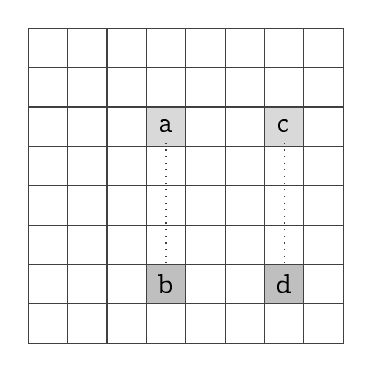
\begin{tikzpicture}
    %\draw[draw=black!75, fill=white] (\x,\y) rectangle ++(0.5,0.5); 
    \fill[color=black!15] (1.5,2.5) +(-.25,-.25) rectangle ++(.25,.25); 
    \draw (1.5,2.5) node (a) {a};
    \fill[color=black!15] (3.0,2.5) +(-.25,-.25) rectangle ++(.25,.25); 
    \draw (3.0,2.5) node (c) {c};
    \fill[color=black!25] (1.5,0.5) +(-.25,-.25) rectangle ++(.25,.25); 
    \draw (1.5,0.5) node (b) {b};
    \fill[color=black!25] (3.0,0.5) +(-.25,-.25) rectangle ++(.25,.25); 
    \draw (3.0,0.5) node (d) {d};
    
    \foreach \y in {0,0.5,...,3.5} {
        \foreach \x in {0,0.5,...,3.5} {
          \draw[draw=black!75, fill=white, fill opacity=0.0] (\x,\y) +(-.25,-.25) rectangle ++(.25,.25); 
        }
    }
    \draw[draw=black!75,dotted] (a) -- (b);
    \draw[draw=black!75,dotted] (c) -- (d);
  \end{tikzpicture}
  \end{center}
  \end{minipage}
  \begin{minipage}[c]{0.67\linewidth}
  % $\forall \;a=A[i_1][j_1], b=A[i_2][j_1], c=A[i_1][j_2], d=A[i_2][j_2]$,\\
  % 其中 $i_1<i_2, j_1<j_2$:

  % FIXME: temporary paragraph spacing hack, fix if possible
  \setlength{\abovedisplayskip}{0pt}
  \setlength{\belowdisplayskip}{0pt}
  凹單調(concave totally monotone):
  $$a\leq b \Rightarrow c\leq d$$

  凸單調(convex totally monotone):
  $$a\geq b \Rightarrow c\geq d$$
  \end{minipage}
  \end{figure}

\end{frame}

\begin{frame}{\btitle{單調性}}
  \begin{itemize}
    \item 假設 $i_1 < i_2, j_1 < j_2$:
    \item 凹單調:若 $A[i_1][j_1] \leq A[i_2][j_1]$ 則 $A[i_1][j_2] \leq A[i_2][j_2]$
    \item 凸單調:若 $A[i_1][j_1] \geq A[i_2][j_1]$ 則 $A[i_1][j_2] \geq A[i_2][j_2]$
    \item 代表最佳選擇具有某種程度的「淘汰性」,也就是某個時間點後一個選擇一旦輸給了某個順序在他之前/後的選擇,他就再也不可能是最佳的選擇
  \end{itemize}
\end{frame}


\begin{frame}{\btitle{凹單調}}
  \begin{figure}[h]
  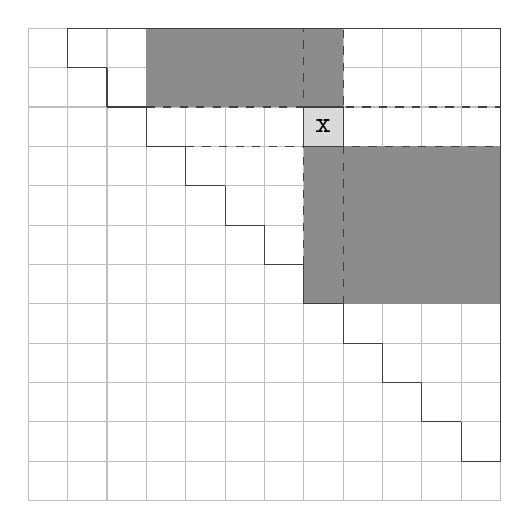
\begin{tikzpicture}
    \foreach \y in {0,0.5,...,5.5} {
        \foreach \x in {0,0.5,...,5.5} {
        \pgfmathsetmacro{\sumxy}{\x+\y};
            \ifthenelse{\lengthtest{\sumxy pt<5.6pt}}{
              \draw[draw=black!10, fill=white] (\x,\y) rectangle ++(0.5,0.5); 
            } {
                \draw[draw=black!25, fill=white] (\x,\y) rectangle ++(0.5,0.5); 
            }
        }
    }
    %
    \foreach \x in {3.5,4.0,...,5.5} {
        \foreach \y in {2.5,3.0,...,4.0} {
        \pgfmathsetmacro{\sumxy}{\x+\y};
            \ifthenelse{\lengthtest{\sumxy pt<5.6pt}}{
            } {
                \draw[draw opacity=0, fill=black!45] (\x,\y) rectangle ++(0.5,0.5); 
            }
        }
    }
    \foreach \x in {1.5,2.0,...,3.5} {
        \foreach \y in {5.0,5.5} {
        \pgfmathsetmacro{\sumxy}{\x+\y};
            \ifthenelse{\lengthtest{\sumxy pt<5.6pt}}{
            } {
                \draw[draw opacity=0, fill=black!45] (\x,\y) rectangle ++(0.5,0.5); 
            }
        }
    }
    %
    \draw[draw=black!75] (0.5,6) -- (6,6);
    \draw[draw=black!75] (6,0.5) -- (6,6);
    \foreach \x in {0.5,1.0,...,5.5} {
      \draw[draw=black!75] (\x,6.5-\x) -- (\x,6.0-\x);
      \draw[draw=black!75] (\x,6.0-\x) -- (\x+0.5,6.0-\x);
    }
    \draw[draw=black!75,dashed] (3.5,3.0) -- (3.5,6.0);
    \draw[draw=black!75,dashed] (4.0,2.5) -- (4.0,6.0);
    \draw[draw=black!75,dashed] (1.5,5.0) -- (6.0,5.0);
    \draw[draw=black!75,dashed] (2.0,4.5) -- (6.0,4.5);
    \draw[draw=black!75,fill=black!15] (3.5,4.5) rectangle ++(0.5,0.5);
    \draw (3.75,4.75) node (x) {x};
  \end{tikzpicture}
  \caption{凹單調時,被 x 殺死的元素}
  \end{figure}
\end{frame}

\begin{frame}{\btitle{凹單調}}
  \begin{figure}[h]
  \begin{tikzpicture}
    \foreach \y in {0,0.5,...,5.5} {
        \foreach \x in {0,0.5,...,5.5} {
        \pgfmathsetmacro{\sumxy}{\x+\y};
          %\ifthenelse{\lengthtest{\sumxy pt<5.4pt}}{\def\mycol{black!15}}{\def\mycol{white}}
            %\draw[draw=black!75, fill=\mycol] (\x,\y) rectangle ++(0.5,0.5); 
            \ifthenelse{\lengthtest{\sumxy pt<5.6pt}}{
              \draw[draw=black!10, fill=white] (\x,\y) rectangle ++(0.5,0.5); 
            } {
                \draw[draw=black!25, fill=white] (\x,\y) rectangle ++(0.5,0.5); 
            }
        }
    }
    \draw[draw=black!75] (0.5,6) -- (6,6);
    \draw[draw=black!75] (6,0.5) -- (6,6);
    \foreach \x in {0.5,1.0,...,5.5} {
      \draw[draw=black!75] (\x,6.5-\x) -- (\x,6.0-\x);
      \draw[draw=black!75] (\x,6.0-\x) -- (\x+0.5,6.0-\x);
    }
    \draw[draw=black!75,dashed] (3.0,3.5) -- (3.0,6.0);
    \draw[draw=black!75,dashed] (3.0,3.5) -- (6.0,3.5);
    \draw[draw=black!75,fill=black!15] (3.0,3.0) rectangle (3.5,3.5);
    \draw[draw=black!75,fill=white,fill opacity=0.6] (3.0,3.5) rectangle (4.5,4.0);
    \draw[draw=black!75,fill=black,draw opacity=0.4,fill opacity=0.1] (4.0,3.5) rectangle (4.5,4.0);
    \draw[draw=black!75,fill=white,fill opacity=0.6] (4.5,4.5) rectangle (5.0,5.0);
    \draw[draw=black!75,fill=black,draw opacity=0.4,fill opacity=0.1] (4.5,4.5) rectangle (5.0,5.0);
    \draw[draw=black!75,fill=white,fill opacity=0.6] (5.0,5.0) rectangle (6.0,5.5);
    \draw[draw=black!75,fill=black,draw opacity=0.4,fill opacity=0.1] (5.5,5.0) rectangle (6.0,5.5);
    %
    \node [anchor=east] at (0,3.25) {$j-1$};
    \node [anchor=east] at (0,3.75) {$i_1$};
    \node [anchor=east] at (0,4.75) {$\vdots$};
    \node [anchor=east] at (0,5.25) {$i_r$};
    %
    \node [anchor=south] at (3.25,6) {$j$};
    \node [anchor=south] at (4.25,6) {$h_1$};
    \node [anchor=south] at (4.75,6) {$\cdots$};
    \node [anchor=south] at (5.75,6) {$h_r$};
  \end{tikzpicture}
  \caption{凹單調性 DP}
  \end{figure}
\end{frame}

\begin{frame}{\btitle{凹單調}}
  \begin{itemize}
    \item 用\textbf{列區間(row segment)}來代表這些人選
    \item $S = ([i_1,j:h_1],[i_2,h_1+1:h_2],\dots,[i_k,h_{k-1}+1:h_k])$
    \item 其中 $[i,j_1:j_2]$ 代表第 $i$ 列上,第 $j_1$ 到第 $j_2$ 行所形成的列區間,$h_t$ 是第 $t$ 個列區間的最右元素
  \end{itemize}
\end{frame}

\begin{frame}[fragile]{\btitle{凹單調}}
  \begin{minted}[breaklines]{cpp}
    stack<Seg> sta;
    sta.push(Seg(0, 1, m));
    for (int j = 1; j <= m; ++j) {
      while (!sta.empty() && sta.top().r < j) sta.pop(); // 把過期的最佳解丟掉
      dp[j] = cal(sta.top().pos, j);
      
      while (!sta.empty() && cal(sta.top().pos, sta.top().r) > cal(j, sta.top().r)) {
        // 把被完全覆蓋的線段刪掉
        sta.pop();
      }
      if (sta.empty()) {
        sta.push(Seg(j, j + 1, m));
      }
  \end{minted}
\end{frame}

\begin{frame}[fragile]{\btitle{凹單調}}
  \begin{minted}[breaklines]{cpp}
      else {
        Seg seg = sta.top(); sta.pop();
        // 二分搜斷點
        int l = seg.l - 1, r = seg.r;
        while (r - l > 1) {
          int mid = (l + r) >> 1;
          if (cal(seg.pos, mid) >= cal(j, mid)) l = mid;
          else r = mid;
        }
        sta.push(Seg(seg.pos, r, seg.r));
        if (j + 1 <= l) sta.push(Seg(j, j + 1, l));
      }
    }
  \end{minted}
\end{frame}



\begin{frame}{\btitle{凸單調}}
  \begin{figure}[h]
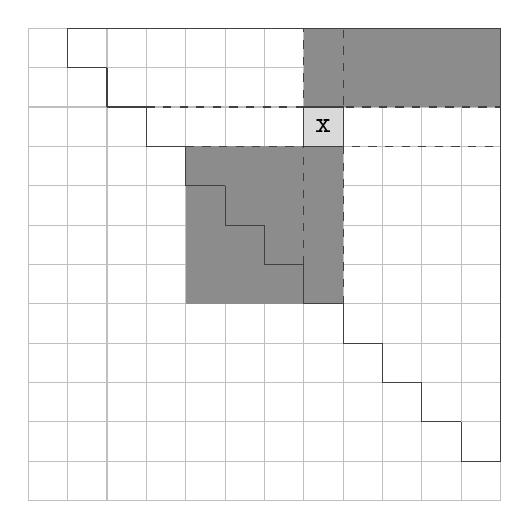
\begin{tikzpicture}
  \foreach \y in {0,0.5,...,5.5} {
      \foreach \x in {0,0.5,...,5.5} {
      \pgfmathsetmacro{\sumxy}{\x+\y};
          \ifthenelse{\lengthtest{\sumxy pt<5.6pt}}{
            \draw[draw=black!10, fill=white] (\x,\y) rectangle ++(0.5,0.5); 
          } {
              \draw[draw=black!25, fill=white] (\x,\y) rectangle ++(0.5,0.5); 
          }
      }
  }
  %
  \foreach \x in {2.0,2.5,...,3.5} {
      \foreach \y in {2.5,3.0,...,4.0} {
      \pgfmathsetmacro{\sumxy}{\x+\y};
          \ifthenelse{\lengthtest{\sumxy pt<5.6pt}}{
          } {
              \draw[draw opacity=0, fill=black!45] (\x,\y) rectangle ++(0.5,0.5); 
          }
      }
  }
  \foreach \x in {3.5,4,...,5.5} {
      \foreach \y in {5.0,5.5} {
          \draw[draw opacity=0, fill=black!45] (\x,\y) rectangle ++(0.5,0.5); 
      }
  }
  %
  \draw[draw=black!75] (0.5,6) -- (6,6);
  \draw[draw=black!75] (6,0.5) -- (6,6);
  \foreach \x in {0.5,1.0,...,5.5} {
    \draw[draw=black!75] (\x,6.5-\x) -- (\x,6.0-\x);
    \draw[draw=black!75] (\x,6.0-\x) -- (\x+0.5,6.0-\x);
  }
  \draw[draw=black!75,dashed] (3.5,3.0) -- (3.5,6.0);
  \draw[draw=black!75,dashed] (4.0,2.5) -- (4.0,6.0);
  \draw[draw=black!75,dashed] (1.5,5.0) -- (6.0,5.0);
  \draw[draw=black!75,dashed] (2.0,4.5) -- (6.0,4.5);
  \draw[draw=black!75,fill=black!15] (3.5,4.5) rectangle ++(0.5,0.5);
  \draw (3.75,4.75) node (x) {x};
\end{tikzpicture}  \caption{凸單調時,被 x 殺死的元素}
  \end{figure}
\end{frame}

\begin{frame}{\btitle{凸單調}}
  \begin{figure}[h]
\begin{tikzpicture}
  \foreach \y in {0,0.5,...,5.5} {
      \foreach \x in {0,0.5,...,5.5} {
      \pgfmathsetmacro{\sumxy}{\x+\y};
        %\ifthenelse{\lengthtest{\sumxy pt<5.4pt}}{\def\mycol{black!15}}{\def\mycol{white}}
          %\draw[draw=black!75, fill=\mycol] (\x,\y) rectangle ++(0.5,0.5); 
          \ifthenelse{\lengthtest{\sumxy pt<5.6pt}}{
            \draw[draw=black!10, fill=white] (\x,\y) rectangle ++(0.5,0.5); 
          } {
              \draw[draw=black!25, fill=white] (\x,\y) rectangle ++(0.5,0.5); 
          }
      }
  }
  \draw[draw=black!75] (0.5,6) -- (6,6);
  \draw[draw=black!75] (6,0.5) -- (6,6);
  \foreach \x in {0.5,1.0,...,5.5} {
    \draw[draw=black!75] (\x,6.5-\x) -- (\x,6.0-\x);
    \draw[draw=black!75] (\x,6.0-\x) -- (\x+0.5,6.0-\x);
  }
  \draw[draw=black!75,dashed] (3.0,3.5) -- (3.0,6.0);
  \draw[draw=black!75,dashed] (3.0,3.5) -- (6.0,3.5);
  \draw[draw=black!75,fill=black!15] (3.0,3.0) rectangle (3.5,3.5);
  \draw[draw=black!75,fill=white,fill opacity=0.6] (3.0,5.5) rectangle (3.5,6.0);
  \draw[draw=black!75,fill=black,draw opacity=0.4,fill opacity=0.1] (3.0,5.5) rectangle (3.5,6.0);
  \draw[draw=black!75,fill=white,fill opacity=0.6] (3.5,5.0) rectangle (4.0,5.5);
  \draw[draw=black!75,fill=black,draw opacity=0.4,fill opacity=0.1] (3.5,5.0) rectangle (4.0,5.5);
  \draw[draw=black!75,fill=white,fill opacity=0.6] (4.0,4.5) rectangle (5.5,5.0);
  \draw[draw=black!75,fill=black,draw opacity=0.4,fill opacity=0.1] (4.0,4.5) rectangle (4.5,5.0);
  \draw[draw=black!75,fill=white,fill opacity=0.6] (5.5,4.0) rectangle (6.0,4.5);
  \draw[draw=black!75,fill=black,draw opacity=0.4,fill opacity=0.1] (5.5,4.0) rectangle (6.0,4.5);
  %
  \node [anchor=east] at (0,3.25) {$j-1$};
  \node [anchor=east] at (0,5.75) {$i_1$};
  \node [anchor=east] at (0,5.25) {$i_2$};
  \node [anchor=east] at (0,4.75) {$\vdots$};
  \node [anchor=east] at (0,4.25) {$i_r$};
  %
  \node [anchor=south east] at (3.55,6) {$h_1=j$};
  \node [anchor=south] at (3.75,6) {$h_2$};
  \node [anchor=south] at (4.25,6) {$\cdots$};
  \node [anchor=south] at (5.75,6) {$h_r$};
\end{tikzpicture}
  \caption{凸單調性 DP}
  \end{figure}
\end{frame}

\begin{frame}{\btitle{凸單調}}
  \begin{itemize}
    \item 用\textbf{列區間(row segment)}來代表這些人選
    \item $S = ([i_1,j:h_1],[i_2,h_1+1:h_2],\dots,[i_k,h_{k-1}+1:h_k])$
    \item 其中 $[i,j_1:j_2]$ 代表第 $i$ 列上,第 $j_1$ 到第 $j_2$ 行所形成的列區間,$h_t$ 是第 $t$ 個列區間的最右元素
  \end{itemize}
\end{frame}

\begin{frame}[fragile]{\btitle{凸單調}}
  \begin{minted}[breaklines]{cpp}
    deque<Seg> dq;
    dq.push_back(Seg(0, 1, n));
    for (int j = 1; j <= n; ++j) {
      while (!dq.empty() && dq[0].r < j) dq.pop_front(); // 把過期的最佳解丟掉
      dp[j] = cal(dq[0].pos, j);
      while (!dq.empty() && cal(dq.back().pos, dq.back().l) > cal(j, dq.back().l)) {
        // 把被完全覆蓋的線段刪掉
        dq.pop_back();
      }
      if (dq.empty()) {
        dq.push_back(Seg(j, j + 1, n));
      }
  \end{minted}
\end{frame}

\begin{frame}[fragile]{\btitle{凸單調}}
  \begin{minted}[breaklines]{cpp}
      else {
        Seg seg = dq.back(); dq.pop_back();
        // 二分搜斷點
        int l = seg.l, r = seg.r + 1;
        while (r - l > 1) {
          int mid = (l + r) >> 1;
          if (cal(seg.pos, mid) > cal(j, mid)) r = mid;
          else l = mid;
        }
        dq.push_back(Seg(seg.pos, seg.l, l));
        if (l != n) dq.push_back(Seg(j, l + 1, n));
      }
    }
  \end{minted}
\end{frame}

\begin{frame}{\btitle{Monge Condition}}
  \begin{theorem}[Monge condition]
    給一個$m \times n$ 矩陣 $B$,若 $\forall 1\leq i_1<i_2 \leq m, 1\leq j_1<j_2\leq n$我們有:
    $$B[i_1][j_1]+B[i_2][j_2] \;\;\leq (\geq)\;\; B[i_1][j_2]+B[i_2][j_1]$$
    那我我們說他符合 convex (concave) Monge condition.
  \end{theorem}
  \begin{theorem}[Monge condition (等價形式)]
    給一個$m \times n$ 矩陣 $B$,若 $\forall 1\leq i<m, 1\leq j< n$我們有:
    $$B[i][j]+B[i+1][j+1] \;\;\leq (\geq)\;\; B[i][j+1]+B[i+1][j]$$
    那我我們說他符合 convex (concave) Monge condition.
  \end{theorem}
\end{frame}

\begin{frame}{\btitle{Monge Condition}}
  \begin{itemize}
    \item 容易驗證,由 convex (concave) Monge condition 推得凸(凹)單調性(也就是說,凹凸單調優化的正確性常用 Monge condition 證明)
    \item 要注意的是,Monge condition 事實上是比較嚴格的,因此\textbf{反方向的推論並不成立},不符合 Monge condition 也不代表不具有單調性
  \end{itemize}
\end{frame}

\end{document}



\documentclass[standalone]{beamer}

\begin{document}
\section{Knuth Optimization}

\begin{frame}{\btitle{前言}}
  \begin{itemize}
    \item 前面的章節,幾乎都是介紹 1D / 1D 的 DP 優化
    \item 現在要來介紹 2D / 1D 相關的優化
  \end{itemize}
\end{frame}

\begin{frame}{\btitle{問題定義}}
  \begin{theorem}[(2D/1D)]
  要求的是一個二維代價 $dp[i][j], \;\forall\; 1\leq i< j\leq n$。
  給一可在常數時間內求得的轉移代價函數 (transition cost function) $w(i,j), \;\forall\; 1\leq i<j\leq n$、
  及初始化邊界 $dp[i][i]=0, \;\forall\; 1\leq i \leq n$;求:
  %\[ E[j] = \min_{0\leq i<j}\left\{f(i,E[i])+w(i,j)\right\}, \;\forall\; 1\leq i\leq n \]
  \[ dp[i][j] = w(i,j) + \min_{i\leq k<j}\left\{dp[i][k]+dp[k+1][j]\right\}, \;\forall\; 1\leq i<j\leq n \]
  \end{theorem}
\end{frame}

\begin{frame}{\btitle{問題定義}}
  \begin{itemize}
    \item 我們知道 2D/1D 問題有顯然的 $O(N^3)$ 作法
    \item 亦即對於要求 $dp[i][j]$,枚舉 $1\leq k <j$作為轉移的決策點並找到最小的轉移來源
    \item 我們稱在這轉移中的最佳選擇 $k$ 為 $K_{i,j} = \mathrm{argmin}_{i\leq k<j}\left\{dp[i][k]+dp[k+1][j]\right\}$
    \item 這邊我們提出一個性質:Optimal Split Point Monotonicity
  \end{itemize}
\end{frame}

\begin{frame}{\btitle{重要性質}}
  \begin{theorem}[Monge condition implies Monotonic Optimal Split Point]
  當上述 2D/1D 問題的代價 $C$ 滿足凸 convex Monge condition,亦即:
  $$ dp[i][j]+dp[i+1][j+1] \geq dp[i][j+1]+dp[i+1][j]$$
  則決策點具有單調性:
  $$ K_{i,j-1} \leq K_{i,j} \leq K_{i+1,j} $$
  \end{theorem}

  白話來說:$dp[i][j]$ 的決策點界於 $dp[i][j-1]$ 與 $dp[i+1][j]$ 的決策點之間
\end{frame}

\begin{frame}{Knuth Optimization}
  \begin{itemize}
    \item 光這麼看好像看不出什麼端睨,$K_{i,j-1}$ 到 $K_{i+1,j}$ 究竟有多大也不清楚
    \item 不過這時依然可以使用均攤分析!就讓我們一次分析填完一整(斜)排 DP 所需要花的時間吧:

    \[
    \begin{array}{r c l}
               \dots &    \dots    & \dots \\
    K_{i-2,j-3} \leq & K_{i-2,j-2} & \leq K_{i-1,j-2} \\
    K_{i-1,j-2} \leq & K_{i-1,j-1} & \leq K_{i,j-1} \\
    K_{i,j-1}   \leq & K_{i,j}     & \leq K_{i+1,j} \\
    K_{i+1,j}   \leq & K_{i+1,j+1} & \leq K_{i+2,j+1} \\
    K_{i+2,j+1} \leq & K_{i+2,j+2} & \leq K_{i+3,j+2}  \\
               \dots &    \dots    & \dots
    \end{array}
    \]
  \end{itemize}
\end{frame}

\begin{frame}{Knuth Optimization}
  \begin{itemize}
    \item 斜著做 DP 的話,每一列要考慮的數量和不超過 $N$
    \item 總複雜度為 $O(2N \times N) = O(N^2)$
  \end{itemize}
\end{frame}

\begin{frame}[fragile]{\btitle{範例程式碼}}
  \begin{minted}[breaklines]{cpp}
    int kl = K[i][j - 1];
    int kr = K[i + 1][j];
    for (int k = kl; k <= kr; ++k) {
      if (w(i, j) + dp[i][k] + dp[k + 1][j] < dp[i][j]) {
        dp[i][j] = w(i, j) + dp[i][k] + dp[k + 1][j];
        K[i][j] = k;
      }
    }
  \end{minted}
\end{frame}

\begin{frame}{2D / 1D 凹優化}
  \begin{itemize}
    \item 基本上就只是做 $N$ 次 1D / 1D 凹優化
    \item 非常不常見,這邊就不細講
  \end{itemize}
\end{frame}

\end{document}


\documentclass[standalone]{beamer}

\begin{document}
\section{轉移點單調優化}

\begin{frame}{\btitle{例題}}
  \begin{problem}[經典問題]
    令 $F(i, j)$ 為一個對所有 $1 \leq i \leq j \leq N$ 的正整數 $i, j$ 都有定義的函數。對於所有的 $1 \leq j \leq N$,求 $\min_{i \leq j}F(i, j)$ 或 $\max_{i \leq j}F(i, j)$。
  \end{problem}
  這樣看起來有點抽象,我們來實際看一個例子:
\end{frame}

\begin{frame}{\btitle{例題}}
  \begin{problem}[AtCoder ARC067 D Yakiniku Restaurants]
    有 $N$ 個位於一維數線上的餐廳,由左至右編為 $1$ 到 $N$ 號,其中 $i$ 號餐廳與 $i - 1$ 號餐廳的距離為 $A_i$。你有 $M$ 張餐卷,第 $i$ 張可以兌換第 $i$ 種食物且只能使用一次。已知這 $N$ 家餐廳都有販售這 $M$ 種食物,且第 $i$ 家餐廳的第 $j$ 種食物的好吃度為 $B_{i, j}$。你可以從任意間餐廳開始,請問「吃到食物的好吃度總和 $-$ 總行走距離」的最大值為何。
    
    \begin{itemize}
      \item $1 \leq N \leq 5000$
      \item $1 \leq M \leq 200$
    \end{itemize}
  \end{problem}
\end{frame}

\begin{frame}{\btitle{例題}}
  \begin{itemize}
    \item 首先可以知道,當決定了要在哪些餐廳買食物之後,最佳的策略一定是從最左的直接走到最右邊的餐廳,不會來回行走
    \item 因此,定義 $F(i, j)$ 為從 $i$ 號餐廳開始,結束在 $j$ 號餐廳的最大價值。則 $F(i, j)$ 可以被寫成
    \item $F(i, j) = \left(\sum_{f = 1}^{M}\max_{i \leq k \leq j}B_{k, f}\right) - \left(\sum_{k = i + 1}^{j}A_k\right)$
    \item 其中 $i$ 與 $j$ 之間各種食物的最大好吃度可以透過 RMQ 預處理,$i$ 與 $j$ 的距離也可以透過前綴和達到 $O(1)$,因此可以在 $O(M)$ 的時間內計算好 $F(i, j)$
  \end{itemize}
\end{frame}

\begin{frame}{\btitle{例題}}
  那該如何有效率的計算 $\max_{i \leq j}F(i, j)$,或是更一般的,對所有餐廳 $j$ 求出以它當終點的最大價值呢 $V_j$?這裡我們必須用到一個性質:
  \begin{theorem}[性質]
    令 $H_j$ 為以 $j$ 當終點情況下的最佳起點,亦即:

    \[ H_j = \mathop{\arg\max}_{i \leq j}F(i, j) \]

    則 $H_j \leq H_{j + 1}$。也就是說當終點向右時,最佳的起點只會往右或不動(證明是用 Monge Condition 證的)
  \end{theorem}
\end{frame}

\begin{frame}{\btitle{演算法}}
\begin{itemize}
  \item 有了這個性質之後,可以考慮下列的分治算法:
  \item 假設現在我們想要計算所有 $L \leq j \leq R$ 的 $V_j$,並且我們知道所有在範圍內的 $H_j$ 都滿足 $L^\prime \leq H_j \leq R^\prime$ 
  \item 令 $M = \lfloor\frac{L + R}{2}\rfloor$,那我們在 $O(R^\prime - L^\prime)$ 次計算 $F$ 值之內,枚舉 $[L^\prime, \min(R^\prime, M)]$ 之間的 $i$ 並找出最大的 $F(i, j)$ 以及對應的 $H_M$
  \item 根據單調性,我們知道 $[L, M - 1]$ 的最佳起點會落在 $[L^\prime, H_M]$ 、 $[M + 1, R]$ 的最佳起點會落在 $[H_M, R^\prime]$。因此我們分別遞迴計算子問題 $\{L, M - 1, L^\prime, H_M\}$ 及 $\{M + 1, R, H_M, R^\prime\}$
  \item 複雜度為 $O(N \log N \times F())$,其中 $F$ 是算一個 $F(i, j)$ 的值的複雜度
\end{itemize}
\end{frame}

\begin{frame}[fragile]{\btitle{演算法}}
  \begin{minted}[breaklines]{cpp}
    void dc(int L, int R, int best_L, int best_R) {
      if (L > R) return;
      int mid = (L + R) >> 1;
      for (int i = best_L; i <= best_R; ++i) {
        if (h[mid] == 0 || f(mid, i) > f(mid, h[mid])) h[mid] = i;
      }
      dc(L, mid - 1, best_L, h[mid]);
      dc(mid + 1, R, h[mid], best_R);
    }
  \end{minted}
\end{frame}

\begin{frame}{\btitle{CDQ 配轉移點單調}}
  \begin{itemize}
    \item 有了轉移點單調這個好東西後,我們可以回頭看一次 1D / 1D 凸單調
    \item 應該不難發現,\textbf{1D / 1D 凸單調也是具有轉移點單調}這個性質的,但是在有些時候,\textbf{轉移來源必須是在線的},導致我們無法快樂直接套用轉移點單調
    \item 但其實,這個世界並沒有這麼不美好。這個問題可以用類似斜率優化 CDQ 的思維,來多花一點時間解決!假設我們現在正在算 $[L, R]$ 的答案,算法過程如下:
  \end{itemize}
\end{frame}

\begin{frame}{\btitle{CDQ 配轉移點單調}}
  \begin{itemize}
    \item 如果 L == R,結束遞迴
    \item 否則,依序執行以下步驟:
    \begin{itemize}
      \item 遞迴計算左半部 $[L, mid]$ 的 DP 值。
      \item 用左半部 $[L, mid]$ 算出來的 DP 值,更新右半部 $[mid + 1, R]$ 的 DP 值。
      \item 遞迴計算右半部的 $[mid + 1, R]$ DP 值。
    \end{itemize}
    \item 複雜度為 $O(N \log^2 N)$
    \item 範例 code 麻煩參考講義~
  \end{itemize}
\end{frame}

\begin{frame}{\btitle{CDQ 配轉移點單調}}
  \begin{itemize}
  \item 而根據前面的分析,這個演算法的重點會是在「用左半部的 DP 值更新右半部的 DP 值」這個部份上
  \item 而因為我們已經算出左半部的所有的 DP 值,所以這其實本質上就是一個\textbf{代價可以離線的轉移點單調 DP 問題}
  \item 所以,我們可以花 $O(N \log N)$ 的時間,跑一次轉移點單調優化,來達到「用左半部的 DP 值更新右半部的 DP 值」這個部份
  \end{itemize}
\end{frame}

\begin{frame}{\btitle{基於轉移點單調的唬爛}}
  \begin{itemize}
    \item 使用這個方法之前,要先決定一個魔法常數 $magic$,接著,該方法的執行過程如下:
    \item 假設現在在計算 $dp(i)$,並已知 $dp(i - 1)$ 的轉移點為 $p$
    \item 嘗試從 $[p, p + magic]$ 轉移到 $dp(i)$,如果發現一個比 $p$ 好的點,把 $p$ 更新成新的轉移點,並重新執行這部份
    \item 嘗試從 $[i - magic, i]$ 轉移到 $dp(i)$,如果發現一個比 $p$ 好的點,就更新 $p$
    \item 複雜度為 $O(magic \times N)$,\textbf{但是並沒有保證正確性!}
    \item 但是不失為一個\textbf{唬爛好方法}
  \end{itemize}
\end{frame}


\end{document}


\documentclass[standalone]{beamer}

\begin{document}
\section{SMAWK 演算法}

\begin{frame}{\btitle{前言}}
  \begin{itemize}
    \item 前面的轉移點單調,已經讓複雜度從 $O(N^2)$ 的東西壓到 $O(N \log N)$
    \item 現在,要來進一步的壓到 $O(N)$
  \end{itemize}
\end{frame}

\begin{frame}{\btitle{定義}}
  \begin{theorem}
    定義一個 $2 \times 2$ 矩陣 $\begin{bmatrix}
      a & b \\
      c & d
    \end{bmatrix}$ 是單調的,如果以下兩個條件都有成立:

    \begin{itemize}
      \item 如果 $c < d$,那麼 $a < b$
      \item 如果 $c = d$,那麼 $a \leq b$
    \end{itemize}

    而一個 $N \times M$ 的矩陣是 \textbf{完全單調矩陣},若且唯若每個 $2 \times 2$ 的子矩陣(submatrix)都是單調矩陣。注意到子矩陣的列(row),行(column)不一定要是連續的。
  \end{theorem}

  定義 $h(i)$ 是第 $i$ 列中,最左邊最小值發生的位置。而如果 $N \times M$ 的矩陣 $A$ 是一個完全單調矩陣,那麼會有 $h(1) \leq h(2) \leq \dots \leq h(N)$ 這個性質
\end{frame}

\begin{frame}{SMAWK 演算法}
  \begin{itemize}
    \item 而 SMAWK 演算法做的事情,就是給定一個 $N \times M$ 大小的完全單調矩陣,SMAWK 演算法會在 $O(N + M)$ 的時間內,找到 $h(1), h(2), \dots, h(N)$
    \item 這個演算法分成的架構如下:
    \begin{itemize}
      \item 若 $\max(N, M) \leq 2$,暴力算出所有的 $h(i)$。
      \item 若 $N \geq M$,則呼叫 \texttt{interpolate()} 算法,遞迴計算 $\frac{N}{2} \times M$ 矩陣的答案後,找出剩下 $\frac{N}{2}$ 列的答案。
      \item 若 $N < M$,則呼叫 \texttt{reduce()} 算法,把一些不重要的行(column)刪掉後,遞迴呼叫剩下 $N \times N$ 矩陣的答案。
    \end{itemize}
  \end{itemize}
\end{frame}

\begin{frame}{\btitle{interpolate}}
  \begin{itemize}
    \item interpolate 的想法很簡單:把 $N \times M$ 的矩陣分成奇數列與偶數列,把偶數列構成的矩陣拿去遞迴算答案
    \item 當我們有偶數列的答案後,我們就可以根據偶數列的答案,算出奇數列的答案
    \item 根據前面提到的 $h(1) \leq h(2) \leq \dots \leq h(N)$ 的性質,假設我要算奇數列 $h(i)$ 的答案,我們可以發現:$h(i - 1) \leq h(i) \leq h(i + 1)$。也就是說,這個奇數列答案的位置,\textbf{是被前後兩個偶數列的答案位置限制住的}。所以,我們只要跑過 $h(i - 1)$ 到 $h(i + 1)$ 的所有值,就可以知道第 $i$ 行的最小值發生的位置
    \item 也因此,我們就可以花 $O(N + M)$ 加上額外遞迴的時間,完成 interpolate 這個操作。
  \end{itemize}
\end{frame}

\begin{frame}{\btitle{reduce}}
  \begin{itemize}
  \item reduce 這個函數的想法,就是利用矩陣是完全單調的性質,刪掉至少 $M - N$ 個列,讓新的矩陣變成至多 $N \times N$ 後,拿去跑 interpolate
  \item 基本上,會開一個 stack $S$ 來維護要選擇的列。接著,我們會由左而右的看每個列的狀況。假設我們正在看列 $C$,而矩陣的第 $i$ 行第 $j$ 列的值為 $A_{i, j}$。演算法進行過程如下:
  \item 如果 stack 是空的,直接把 $C$ 放進去 stack 裡面。
  \item 否則,執行以下迴圈直到 $S$ 是空的,或者是 $C$ 被擊敗了:
  \begin{itemize}
    \item 假設 stack 裡面有 $x$ 個列,最後一個為 $c_x$。
    \item 如果 $A_{x, c_x} > A_{x, C}$,那麼把 $c_x$ 這列從 stack 中丟掉,因為 $c_x$ 不可能包含最佳解了。
    \item 否則,代表 $C$ 被擊敗了,離開迴圈。
  \end{itemize}
  \item 如果這時候 stack 裡面的列數量小於 $N$ 個,那麼就把 $C$ 丟進 stack 裡面。
\end{itemize}
\end{frame}

\begin{frame}{\btitle{範例}}
  \begin{center}
    \begin{tabular}{|p{0.1\textwidth}|p{0.1\textwidth}|p{0.1\textwidth}|p{0.1\textwidth}|p{0.1\textwidth}|}
      \hline
      10 & 20 & 13 & 19 & 35 \\ [3ex]
      \hline
      20 & 29 & 21 & 25 & 37 \\ [3ex]
      \hline
      28 & 33 & 24 & 28 & 40 \\ [3ex]
      \hline
      42 & 44 & 35 & 38 & 48 \\ [3ex]
      \hline
      48 & 49 & 39 & 42 & 48 \\ [3ex]
      \hline
      56 & 55 & 44 & 44 & 49 \\ [3ex]
      \hline
      75 & 73 & 59 & 57 & 53 \\ [3ex]
      \hline
    \end{tabular}
  \end{center}
\end{frame}

\begin{frame}{\btitle{範例}}
  \begin{center}
    \begin{tabular}{|p{0.1\textwidth}|p{0.1\textwidth}|p{0.1\textwidth}|p{0.1\textwidth}|p{0.1\textwidth}|}
      \hline
       &  &  &  &  \\ [3ex]
      \hline
      20 & 29 & 21 & 25 & 37 \\ [3ex]
      \hline
       &  &  &  &  \\ [3ex]
      \hline
      42 & 44 & 35 & 38 & 48 \\ [3ex]
      \hline
       &  &  &  &  \\ [3ex]
      \hline
      56 & 55 & 44 & 44 & 49 \\ [3ex]
      \hline
       &  &  &  &  \\ [3ex]
      \hline
    \end{tabular}
  \end{center}
\end{frame}

\begin{frame}{\btitle{範例}}
  \begin{center}
    \begin{tabular}{|p{0.1\textwidth}|p{0.1\textwidth}|p{0.1\textwidth}|p{0.1\textwidth}|p{0.1\textwidth}|}
      \hline
       &  &  &  &  \\ [3ex]
      \hline
      \textbf{20} &  & 21 & 25 &  \\ [3ex]
      \hline
       &  &  &  &  \\ [3ex]
      \hline
      42 &  & \textbf{35} & 38 &  \\ [3ex]
      \hline
       &  &  &  &  \\ [3ex]
      \hline
      56 &  & \textbf{44} & 44 &  \\ [3ex]
      \hline
       &  &  &  &  \\ [3ex]
      \hline
    \end{tabular}
  \end{center}
\end{frame}

\begin{frame}{\btitle{範例}}
  \begin{center}
    \begin{tabular}{|p{0.1\textwidth}|p{0.1\textwidth}|p{0.1\textwidth}|p{0.1\textwidth}|p{0.1\textwidth}|}
      \hline
      10 & 20 & 13 & 19 & 35 \\ [3ex]
      \hline
      \textbf{20} & 29 & 21 & 25 & 37 \\ [3ex]
      \hline
      28 & 33 & 24 & 28 & 40 \\ [3ex]
      \hline
      42 & 44 & \textbf{35} & 38 & 48 \\ [3ex]
      \hline
      48 & 49 & 39 & 42 & 48 \\ [3ex]
      \hline
      56 & 55 & \textbf{44} & 44 & 49 \\ [3ex]
      \hline
      75 & 73 & 59 & 57 & 53 \\ [3ex]
      \hline
    \end{tabular}
  \end{center}
\end{frame}


\begin{frame}{\btitle{範例}}
  \begin{center}
    \begin{tabular}{|p{0.1\textwidth}|p{0.1\textwidth}|p{0.1\textwidth}|p{0.1\textwidth}|p{0.1\textwidth}|}
      \hline
      \textbf{10} & 20 & 13 & 19 & 35 \\ [3ex]
      \hline
      \textbf{20} & 29 & 21 & 25 & 37 \\ [3ex]
      \hline
      28 & 33 & \textbf{24} & 28 & 40 \\ [3ex]
      \hline
      42 & 44 & \textbf{35} & 38 & 48 \\ [3ex]
      \hline
      48 & 49 & \textbf{39} & 42 & 48 \\ [3ex]
      \hline
      56 & 55 & \textbf{44} & 44 & 49 \\ [3ex]
      \hline
      75 & 73 & 59 & 57 & \textbf{53} \\ [3ex]
      \hline
    \end{tabular}
  \end{center}
\end{frame}

\begin{frame}{\btitle{時間複雜度}}
  \begin{itemize}
    \item 假設我們拿到一個 $N \times M$ 的矩陣,可以發現大致上需要按照 reduce, interpolate, reduce, interpolate 的順序來執行 SMAWK 演算法
    \item 遞迴式為 $T(N, M) = O(N + M) + T(\frac{N}{2}, N)$
    \item 展開之後可以發現 $T(N, M) = O(M) + 2(O(N) + O(\frac{N}{2}) + O(\frac{N}{4}) + \dots)$,可以發現這是一個 $O(N + M)$ 複雜度的演算法
  \end{itemize}
\end{frame}


\begin{frame}{\btitle{應用}}
  \begin{itemize}
    \item 注意到完全單調矩陣的證明,有的時候要直接證很難。但是,別忘記在前面章節提到的,\textbf{如果那個矩陣符合 monge condition,那麼那個矩陣也會是完全單調矩陣}
    \item 讓我們來看一個例題,底下的例題同時也是 SMAWK 演算法被提出的論文中,論文作者提出來的題目
    \begin{problem}
      給定一個 $N$ 個點的凸多邊形。對於凸多邊形上的每個點 $i$,請求出離點 $i$ 最遠的點的編號。

      % $(N \leq 5 \times 10^5)$
      \begin{itemize}
        \item $N \leq 5 \times 10^5$
      \end{itemize}
    \end{problem}
  \end{itemize}
\end{frame}

\begin{frame}{\btitle{應用}}
    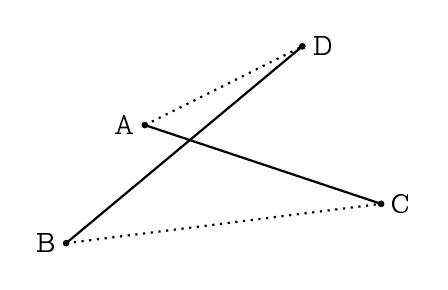
\begin{tikzpicture}[scale=0.5]
\draw[black, thick] (-5, 0) -- (1, 5);
\draw[black, thick] (-3, 3) -- (3, 1);
\draw[black, dotted, thick] (-5, 0) -- (3, 1);
\draw[black, dotted, thick] (-3, 3) -- (1, 5);
\filldraw[black] (-5, 0) circle (2pt) node[anchor=east]{B};
\filldraw[black] (-3, 3) circle (2pt) node[anchor=east]{A};
\filldraw[black] (1, 5) circle (2pt) node[anchor=west]{D};
\filldraw[black] (3, 1) circle (2pt) node[anchor=west]{C};
\end{tikzpicture}

假設 A, B, C, D 這四個點是凸多邊形上按照逆時針順序的四個點。藉由觀察上圖,可以發現 $dis(A, C) + dis(B, D) \geq dis(A, D) + dis(B, C)$。而如果假設那四個點分別是凸多邊形上的第 $x_1, x_2, y_1, y_2$ 個點,就可以把式子寫成 $dis(x_1, y_1) + dis(x_2, y_2) \geq dis(x_2, y_1) + dis(x_1, y_2)$。即可發現這題有「Monge Condition」這個性質
\end{frame}

\end{document}


\documentclass[standalone]{beamer}

\begin{document}
\section{Aliens 優化}

\begin{frame}{\btitle{前言}}
  \begin{itemize}
    \item Aliens 優化又稱 WQS 二分搜,據說在很久之前就在大陸被發明了
    \item 在台灣也會被稱為「帶感情 DP」
    \item 不過使它發揚光大的是 IOI 2016 一道名為 Aliens 的題目
    \item 近幾年基於一些不明的原因開始在臺灣競程界流行了起來,所以在這邊簡單的介紹一下
  \end{itemize}
\end{frame}

\begin{frame}{\btitle{例題}}
  \begin{problem}
    給定一棵 $N$ 個節點的帶權樹以及一個常數 $K$,請找出 $K$ 條邊使得邊權總和最大且不存在兩條邊有共同頂點。

    % $(N \leq 2.5 \times 10^5, K \leq N - 1)$
    \begin{itemize}
      \item $N \leq 2.5 \times 10^5$
      \item $K \leq N - 1$
    \end{itemize}
  \end{problem}
\end{frame}

\begin{frame}{\btitle{例題}}
  先考慮沒有 $K$ 這個限制下要怎麼處理,也就是說找出一些邊使得邊權總和最大且沒有共端點
  
  這是一個經典在樹上 DP 的題目:令(為了方便,定義一個點被選了就是有一條相鄰的邊被選了)

  \begin{align*}
    dp(v, 0) &\coloneqq \text{$v$ 的子樹在 $v$ 還沒有被選的情況下的最大答案} \\
    dp(v, 1) &\coloneqq \text{$v$ 的子樹在 $v$ 被選的情況下的最大答案} \\
  \end{align*} 
\end{frame}

\begin{frame}{\btitle{例題}}
  \begin{itemize}
  % \begin{equation}
    \item $dp(v, 0) = \sum_{(u, w) \in G(v)}\max(dp(u, 0), dp(u, 1))$
    % \end{equation}

    % \begin{equation}
    \item $dp(v, 1) = \max_{(u, w) \in G(v)} \{dp(u, 0) + w +$ $ 
      \sum_{(u^\prime, w^\prime) \in G(v), u^\prime \neq u}\max(dp(u^\prime, 0), dp(u^\prime, 1)) \}$
    % \end{equation}

    \item 其中式子一代表不取 $v$ 向下延伸的邊的 case,所以並不在乎小孩有沒有被選到。而式子二則是枚舉要取哪條邊,所以對應的小孩一定不能被選到,而其他則無所謂。透過一些預處理可以使得這個 DP 算法的複雜度壓到 $O(N)$
    \item 那要怎麼處理有限制個數的狀況呢?其中一個方法是在 DP 狀態多記一個維度代表取了幾條邊,不過會使得複雜度變成至少 $O(NK)$,並不是一個足夠有效率的方法
  \end{itemize}
\end{frame}

\begin{frame}{\btitle{性質}}
  \begin{itemize}
    \item 我們需要以下的性質來幫助解題
    \begin{theorem}[性質]
      令 $f(K)$ 為恰取 $K$ 條邊的最大邊權總和,則 $f$ 是一個凹函數(concave function)\footnote{為了方便說明,這邊指的 concave function 都只定義在整數上面。}。亦即,這個函數滿足 $f(K + 1) - f(K) \leq f(K) - f(K - 1)$。
    \end{theorem}
    \item 也就是 $f$ 的差分遞減。再白話一點的話,就是取第 $K + 1$ 條邊的\textbf{淨獲益}不會比取第 $K$ 條邊的淨獲益來得高(也就是說,隨著 $K$ 的值越來越大,賺到的會越來越少)
    \item 有了這個性質以後,原本的問題就可以被轉為下面的問題
  \end{itemize}
\end{frame}

\begin{frame}{\btitle{性質}}
  \begin{itemize}
    \item 
    \begin{problem}[等價的問題]
      現在有一個凹函數 $f$,我們想知道 $f(K)$ 的值是多少。可惜的是,沒有好的演算法可以直接計算 $f(K)$,可以知道的只有給定 $p$,$f(x) - px$ 的最大值以及最大值發生的位置。要如何運用這些資訊求出 $f(K)$ 呢?
    \end{problem}
    \item 先暫停一下,在給定 $p$ 的情況下,要怎麼算出 $f(x) - px$ 呢?
    \item 如果有一條邊被選擇,我們就額外的扣掉 $p$ 這個邊權
  \end{itemize}
\end{frame}

\begin{frame}{\btitle{性質}}
  \begin{problem}[等價的問題]
    現在有一個凹函數 $f$,我們想知道 $f(K)$ 的值是多少。可惜的是,沒有好的演算法可以直接計算 $f(K)$,可以知道的只有給定 $p$,$f(x) - px$ 的最大值以及最大值發生的位置。要如何運用這些資訊求出 $f(K)$ 呢?
  \end{problem}

  令 $M(p)$ 為 $f(x) - px$ 的最大值,$V(p)$ 為最大值發生的位置,若有多個最大值,則定義為 $x$ 值最小的那個最大值

  不難發現,假設現在我們幸運的找到了一個 $p$,使得 $V(p) = K$,那麼 $f(K)$ 就可以直接用 $f(K) = M(p) + pK$ 算出來了,所以我們的目標就是快速找到這樣的 $p$
\end{frame}

\begin{frame}{\btitle{性質}}
  \begin{itemize}
    \item 令 $M(p)$ 為 $f(x) - px$ 的最大值,$V(p)$ 為最大值發生的位置,若有多個最大值,則定義為 $x$ 值最小的那個最大值
    \item 不妨把 $f(x)$ 的圖形在二維平面上畫出來
    \item 觀察一下後可以知道,$f$ 的長相會長得像一個\textbf{上凸包},且 $V(p) = x$ 就代表存在一條斜率為 $p$ 的直線與 $f$ 的圖形相切於 $(x, f(x))$
    \item 原因是一條斜率為 $p$ 的直線切在 $x$ 上就代表通過 $x$ 這點且斜率為 $p$ 的直線的截距是所有點中最大的
    \item 令切線為 $g(x) = px + b$,則帶入 $(x, f(x))$ 後得到截距 $b = f(x) - px$,恰好與 $M(p)$ 的定義吻合
    \item 不僅如此,當 $x$ 越大時,切在 $(x, f(x))$ 的切線斜率是遞減的。這就告訴我們其實我們可以透過二分搜 $p$ 來找到 $V(p) = K$,再藉此推算 $f(K)$ 
  \end{itemize}
\end{frame}

\begin{frame}{\btitle{性質}}
  \begin{figure}[H]
  \centering
  \begin{tikzpicture}[scale=0.5]
      % Draw axes
      \draw [<->,thick] (0,8) node (yaxis) [above] {$y$}
          |- (18,0) node (xaxis) [right] {$x$};
      \coordinate (f0) at (0, 0);
      \coordinate (f1) at (1, 3);
      \coordinate (f2) at (3, 5);
      \coordinate (f3) at (5, 6);
      \coordinate (f4) at (7, 5.5);
      \coordinate (f5) at (9, 5);
      \coordinate (f6) at (11, 4);
      \coordinate (f7) at (13, 2);
      \coordinate (f8) at (15, 0);

      \draw [thick] (f0) -- (f1);
      \draw [thick] (f1) -- (f2);
      \draw [thick] (f2) -- (f3);
      \draw [thick] (f3) -- (f4);
      \draw [thick] (f4) -- (f5);
      \draw [thick] (f5) -- (f6);
      \draw [thick] (f6) -- (f7);
      \draw [thick] (f7) -- (f8);
      \draw [domain=1:8,smooth,variable=\y,gray] plot ({0.5 * (\y - 1)}, {\y});
      \draw [domain=3:8,smooth,variable=\y,gray] plot ({(\y - 3) * 1.5}, {\y});
      \draw [domain=0:15,smooth,variable=\x,gray] plot ({\x}, {6});
      \draw [domain=2.5:7.25,smooth,variable=\y,gray] plot ({-4 * \y + 29}, {\y});
      \draw [domain=1.5:8,smooth,variable=\y,gray] plot ({(\y - 11.7) / -0.7}, {\y});
      \node at (7, -0.5) (xk) {$x = K$};
      \draw [dashed] (7, 8) -- (7, 0);
      \fill (f0) circle (3pt);
      \fill (f1) circle (3pt);
      \fill (f2) circle (3pt);
      \fill (f3) circle (3pt);
      \fill (f4) circle (3pt);
      \fill (f5) circle (3pt);
      \fill (f6) circle (3pt);
      \fill (f7) circle (3pt);
  \end{tikzpicture}
  \caption{一個可能的 $f(x)$ 以及切線們。注意到切線斜率隨著 $x$ 遞增而遞減,且 $f(x)$ 在 $x = K$ 之處等差。}
  \end{figure}
\end{frame}

\begin{frame}{\btitle{性質}}
  \begin{itemize}
    \item 這邊其實有一個問題,那就是我們可以透過二分搜找到最小的 $p$ 使得 $V(p) \leq k$,但這不保證就真的有那麼一個 $p$ 使得 $V(p) = k$
    \item 不過這件事只會發生在當 $f$ 在 $K \in [V(p), V(p + 1)]$ 之間是等差的情形
    \item 所以一個解決方法是分別求出 $f(V(p))$ 與 $f(V(p + 1))$ 之後內插得到 $f(K)$,也就是說 $f(K) = f(V(p)) + \frac{f(V(p + 1)) - f(V(p))}{V(p + 1) - V(p)}\left(K - V(p)\right)$
\end{itemize}
\end{frame}
\begin{frame}{\btitle{性質}}
\begin{itemize}
    \item 另一種不需要內插的做法用到了 $V(p)$ 定義為最小的最大值發生點以及我們找到的是最小滿足條件的 $p$,在這個情況下,由於 $f(x) - px$ 的頂部是平的,所以我們會有 $f(V(p)) - pV(p) = M(p) = f(K) - pK \implies f(K) = M(p) + pK$
    \item 因此只要找到 $M(p)$ 之後便可以直接找出 $f(K)$ 的值
    \item 一般來說,遇到的題目大部分的 $f$ 都是整數到整數的函數,在這個情況底下 $f$ 形成的凸包的斜率也都會是整數,所以上面講的二分搜以及內插全部都可以在整數上完成,比起使用浮點數計算,在效率以及誤差上會有很大的提升
    \item 另外,這邊並沒有講到合理的二分搜上下界要定在哪,這部分請讀者自行推導一下
  \end{itemize}
\end{frame}

\begin{frame}{\btitle{性質}}
\begin{figure}[H]
\centering
\begin{tikzpicture}[scale=0.5]
    \draw [<->,thick] (0,8) node (yaxis) [above] {$y$}
        |- (18,0) node (xaxis) [right] {$x$};
    \coordinate (f0) at (0, 0);
    \coordinate (f1) at (1, 3.25);
    \coordinate (f2) at (3, 5.75);
    \coordinate (f3) at (5, 7.25);
    \coordinate (f4) at (7, 7.25);
    \coordinate (f5) at (9, 7.25);
    \coordinate (f6) at (11, 6.75);
    \coordinate (f7) at (13, 5.25);
    \coordinate (f8) at (15, 3.75);
    \coordinate (f9) at (17, 0);

    \coordinate (g0) at (0, 0);
    \coordinate (g1) at (1, 3.3);
    \coordinate (g2) at (3, 5.9);
    \coordinate (g3) at (5, 7.5);
    \coordinate (g4) at (7, 7.6);
    \coordinate (g5) at (9, 7.7);
    \coordinate (g6) at (11, 7.3);
    \coordinate (g7) at (13, 5.9);
    \coordinate (g8) at (15, 4.5);
    \coordinate (g9) at (17, 0);

    \draw [thick] (f0) -- (f1);
    \draw [thick] (f1) -- (f2);
    \draw [thick] (f2) -- (f3);
    \draw [thick] (f3) -- (f4);
    \draw [thick] (f4) -- (f5);
    \draw [thick] (f5) -- (f6);
    \draw [thick] (f6) -- (f7);
    \draw [thick] (f7) -- (f8);
    \draw [thick] (f8) -- (f9);

    \draw [gray] (g0) -- (g1);
    \draw [gray] (g1) -- (g2);
    \draw [gray] (g2) -- (g3);
    \draw [gray] (g3) -- (g4);
    \draw [gray] (g4) -- (g5);
    \draw [gray] (g5) -- (g6);
    \draw [gray] (g6) -- (g7);
    \draw [gray] (g7) -- (g8);
    \draw [gray] (g8) -- (g9);

    \node at (7, -0.5) (xk) {$x = K$};
    \draw [dashed] (7, 8) -- (7, 0);

    \fill (f0) circle (3pt);
    \fill (f1) circle (3pt);
    \fill (f2) circle (3pt);
    \fill (f3) circle (3pt);
    \fill (f4) circle (3pt);
    \fill (f5) circle (3pt);
    \fill (f6) circle (3pt);
    \fill (f7) circle (3pt);
    \fill (f8) circle (3pt);
   
\end{tikzpicture}
\caption{$f(x) - px$ 的圖形,其中 $p$ 為最小的 $p$ 使得 $V(p) \leq K$。$x = K$ 之處變為平的。注意到如果二分搜的方向反了(找最大的 $p$ 使得 $V(p) \geq K$ )且 $V(p)$ 的定義不變的話,$f(x) - px$ 會變成淺色的樣子,$x = K$ 的地方就不是平的,直接推 $f(K)$ 便會出錯。}
\end{figure}
\end{frame}

\begin{frame}{\btitle{性質}}
  \begin{itemize}
    \item 回到原題,由於我們已經證明了這題的 $f(x)$ 是凹函數,所以可以套用 Aliens 優化
    \item 而一開始提到的 DP 可以很輕易的被修改成計算 $f(x) - px$ 最大值的形式,只要在取邊相對應的轉移式那邊多扣 $p$ 即可
    \item 至此,我們已經把原本看似高維的問題轉為了一維的問題,而這也是 Aliens 優化最常被使用的地方
    \item 最後要提到的是,大部分的情況下,題目中函數的凹性證明並不會像例題那樣簡單
    \item 據說 IOI 官方也沒有給 Aliens 的證明。所以大部分的時候都是靠感覺,或是本機寫暴力對拍跑跑看小 case 來確認性質
    \item 另外,由於凸函數(convex function)就是凹函數取負,所以上述的所有推導在差分遞增的情況也都成立,修改細節留給讀者自行練習
  \end{itemize}
\end{frame}

\begin{frame}
  感謝大家的聆聽~
\end{frame}

\end{document}


\end{document}

